\documentclass[11pt]{book}
\usepackage[utf8]{inputenc}
\usepackage[english]{babel}
\usepackage{amsmath}
\usepackage{amssymb}
\usepackage{listings}
\usepackage{fancyvrb}
\usepackage{caption}
\usepackage{subcaption}

\usepackage[top=2.5cm, bottom=3cm, left=3.25cm, right=3.25cm, headheight=16pt]{geometry}
\parindent = 0cm
\parskip   = 8pt	%salto de linea

\usepackage{hyperref}
\hypersetup{
    colorlinks=true,
    linkcolor=blue,
    filecolor=magenta,
    urlcolor=blue,
}

\usepackage{graphicx}
\graphicspath{ {images/} }

\title{Machine Learning Lecture Notes}
\author{by Andrew Ng}
\date{Transcripted by: Fernando Garcia de la Cruz}

\begin{document}
\maketitle
\chapter{Week 1}
\section{What is Machine Learning?}
Two definitions of Machine Learning are offered. {\bf Arthur Samuel} described it as: {\bf ``the field of study that gives computers the ability to learn without being explicitly programmed."} This is an older, informal definition.

{\bf Tom Mitchell} provides a more modern definition: 
\begin{quote}
``A computer program is said to learn from experience E with respect to some class of tasks T and performance measure P, if its performance at tasks in T, as measured by P, improves with experience E."
\end{quote}
Example: playing checkers.

E = the experience of playing many games of checkers \\[1pt]
T = the task of playing checkers.\\[1pt]
P = the probability that the program will win the next game.

In general, any machine learning problem can be assigned to one of two broad classifications: {\bf supervised learning, or unsupervised learning}.

\section{Supervised Learning}
In supervised learning, we are given a data set and already know what our correct output should look like, having the idea that there is a relationship between the input and the output.

Supervised learning problems are categorized into ``regression" and ``classification" problems. In a regression problem, we are trying to predict results within a continuous output, meaning that we are trying to map input variables to some continuous function. In a classification problem, we are instead trying to predict results in a discrete output. In other words, we are trying to map input variables into discrete categories. Here is a description on Math is Fun on Continuous and Discrete Data.
\subsection{Example 1}
Given data about the size of houses on the real estate market, try to predict their price. Price as a function of size is a continuous output, so this is a regression problem.

We could turn this example into a classification problem by instead making our output about whether the house ``sells for more or less than the asking price." Here we are classifying the houses based on price into two discrete categories.
\subsection{Example 2}
\begin{itemize}
	\item[A)] {\bf Regression} - Given a picture of Male/Female, We have to predict his/her age on the basis of given picture.
	\item[B)] {\bf Classification}  - Given a picture of Male/Female, We have to predict whether He/She is of High school, College, Graduate age. Another Example for Classification - Banks have to decide whether or not to give a loan to someone on the basis of his credit history.
\end{itemize}
\section{Unsupervised Learning}
Unsupervised learning, on the other hand, allows us to approach problems with little or no idea what our results should look like. We can derive structure from data where we don't necessarily know the effect of the variables.

We can derive this structure by clustering the data based on relationships among the variables in the data.

With unsupervised learning there is no feedback based on the prediction results, i.e., {\bf there is no teacher to correct you}.
\subsection{Example}
{\bf Clustering}: Take a collection of 1000 essays written on the US Economy, and find a way to automatically group these essays into a small number that are somehow similar or related by different variables, such as word frequency, sentence length, page count, and so on.

{\bf Non-clustering}: The ``Cocktail Party Algorithm", which can find structure in messy data (such as the identification of individual voices and music from a mesh of sounds at a \href{https://en.wikipedia.org/wiki/Cocktail_party_effect}{cocktail party}) . Here is an answer on Quora to enhance your understanding: \href{https://www.quora.com/What-is-the-difference-between-supervised-and-unsupervised-learning-algorithms}{click here!}.

\section{ML:Linear Regression with One Variable}
\subsection{Model Representation}
Recall that in regression problems, we are taking input variables and trying to fit the output onto a continuous expected result function.

Linear regression with one variable is also known as ``univariate linear regression".

Univariate linear regression is used when you want to predict a {\bf single output} value y from a {\bf single input} value x. We're doing {\bf supervised learning} here, so that means we already have an idea about what the input/output cause and effect should be.
\subsection{The Hypothesis Function}
Our hypothesis function has the general form:
\begin{equation}
\hat{y} = h_\theta(x) = \theta_0 + \theta_1 x
\end{equation}
Note that this is like the equation of a straight line. We give to $h_\theta(x)$ values for $\theta_0 $ and $\theta_1$ to get our estimated output  output $\hat{y}$ In other words, we are trying to create a function called $h_\theta$ that is trying to map our input data (the x's) to our output data (the y's).

Example:\\
Suppose we have the following set of training data:
\begin{center}
\begin{tabular}{|c|c|}
\hline 
{\bf Input $x$} & {\bf Output $y$} \\ 
\hline 
0 & 4 \\ 
\hline 
1 & 7 \\ 
\hline 
2 & 7 \\ 
\hline 
3 & 8 \\ 
\hline 
\end{tabular}
\end{center} 
Now we can make a random guess about our $h_\theta$ function $\theta_0 = 2$ and $\theta_1 = 2$. The hypothesis function becomes $h_\theta = 2 + 2x$

So for input of 1 to our hypothesis, y will be 4. This is off by 3. Note that we will be trying out various values of $\theta_0$ and $\theta_1$ to try to find values which provide the best possible "fit" or the most representative ``straight line" through the data points mapped on the x-y plane.

\subsection{Cost Function}
We can measure the accuracy of our hypothesis function by using a {\bf cost function}. This takes an average (actually a fancier version of an average) of all the results of the hypothesis with inputs from x's compared to the actual output y's.
\begin{equation}
J(\theta_0, \theta_1) = \frac{1}{2m} \sum_{i=1}^m \left( \hat{y}_{i}- y_{i} \right)^2  = \frac{1}{2m} \sum_{i=1}^m \left( h_\theta (x_{i}) - y_{i} \right)^2
\end{equation}
To break it apart, it is $\frac{1}{2} \bar{x}$ where $\bar{x}$ is the mean of the squares of $(h_\theta (x_{i}) - y_{i})$, or the difference between the predicted value and the actual value.

This function is otherwise called the {\bf ``Squared error function"}, or {\bf ``Mean squared error"}. The mean is halved $\left(\frac{1}{2m}\right)$ as a convenience for the computation of the gradient descent, as the derivative term of the square function will cancel out the $\frac{1}{2}$ term.

Now we are able to concretely measure the accuracy of our predictor function against the correct results we have so that we can predict new results we don't have.

If we try to think of it in visual terms, our training data set is scattered on the x-y plane. We are trying to make straight line (defined by $h_\theta(x)$) which passes through this scattered set of data. Our objective is to get the best possible line. The best possible line will be such so that the average squared vertical distances of the scattered points from the line will be the least. In the best case, the line should pass through all the points of our training data set. In such a case the value of $J(\theta_0, \theta_1)$ will be 0.
\section{ML: Gradient Descent}
So we have our hypothesis function and we have a way of measuring how well it fits into the data. Now we need to estimate the parameters in hypothesis function. That's where gradient descent comes in.

Imagine that we graph our hypothesis function based on its fields $\theta_0$ and $\theta_1$ (actually we are graphing the cost function as a function of the parameter estimates). This can be kind of confusing; we are moving up to a higher level of abstraction. We are not graphing x and y itself, but the parameter range of our hypothesis function and the cost resulting from selecting particular set of parameters.

We put $\theta_0$ on the x axis and $\theta_1$ on the y axis, with the cost function on the vertical z axis. The points on our graph will be the result of the cost function using our hypothesis with those specific theta parameters.

We will know that we have succeeded when our cost function is at the very bottom of the pits in our graph, i.e. when its value is the minimum.

The way we do this is by taking the derivative (the tangential line to a function) of our cost function. The slope of the tangent is the derivative at that point and it will give us a direction to move towards. We make steps down the cost function in the direction with the steepest descent, and the size of each step is determined by the parameter $\alpha$, which is called the learning rate.

The gradient descent algorithm is:
\begin{align*}
  \text{repeat until convergence: } \lbrace & \\
\theta_j := \theta_j - \alpha \frac{\partial}{\partial \theta_j} J(\theta_0, \theta_1)
  \\
  \rbrace &
\end{align*}
where

j=0,1 represents the feature index number.

Intuitively, this could be thought of as:

repeat until convergence:

\[\
\theta_j := -\alpha \delta
\]
where: $\delta = \text{[Slope of tangent aka derivative in j dimension]}$
\subsection{Gradient Descent for Linear Regression}
When specifically applied to the case of linear regression, a new form of the gradient descent equation can be derived. We can substitute our actual cost function and our actual hypothesis function and modify the equation to (the derivation of the formulas are out of the scope of this course, but a really great one can be found here):
\begin{align*}
  \text{repeat until convergence: } \lbrace & \\
  \theta_0 := & \theta_0 - \alpha \frac{1}{m} \sum\limits_{i=1}^{m}(h_\theta(x_{i}) - y_{i}) \\
  \theta_1 := & \theta_1 - \alpha \frac{1}{m} \sum\limits_{i=1}^{m}\left((h_\theta(x_{i}) - y_{i}) x_{i}\right) \\
  \rbrace &
\end{align*}
where m is the size of the training set, $\theta_0$ a constant that will be changing simultaneously with $\theta_1$ and $x_{i}$, $y_{i}$ are values of the given training set (data).

Note that we have separated out the two cases for $\theta_j$ into separate equations for $\theta_0 $ and $\theta_1$; and that for $\theta_1$ we are multiplying $x_{i}$ at the end due to the derivative.

The point of all this is that if we start with a guess for our hypothesis and then repeatedly apply these gradient descent equations, our hypothesis will become more and more accurate.
\subsection{Gradient Descent for Linear Regression: visual worked example}
Some may find the following \href{https://www.youtube.com/watch?v=WnqQrPNYz5Q}{video} useful as it visualizes the improvement of the hypothesis as the error function reduces.
\section{ML:Linear Algebra Review}
Khan Academy has excellent Linear Algebra Tutorials: \href{https://www.khanacademy.org/#linear-algebra}{click here!}
\subsection{Matrices and Vectors}
Matrices are 2-dimensional arrays:
\[
\begin{bmatrix}  
a & b & c \\   
d & e & f \\   
g & h & i \\   
j & k & l
\end{bmatrix}
\]
The above matrix has four rows and three columns, so it is a 4 x 3 matrix.

A vector is a matrix with one column and many rows:
\[
\begin{bmatrix}  
w \\  
x \\
y \\
z 
\end{bmatrix}
\]
So vectors are a subset of matrices. The above vector is a 4 x 1 matrix.

{\bf Notation and terms:}
\begin{itemize}
	\item $A_{ij}$ refers to the element in the ith row and jth column of matrix A.
	\item A vector with `n' rows is referred to as an `n'-dimensional vector
	\item $v_i$ refers to the element in the ith row of the vector.
	\item In general, all our vectors and matrices will be 1-indexed. Note that for some programming languages, the arrays are 0-indexed.
	\item Matrices are usually denoted by uppercase names while vectors are lowercase.
	\item ``Scalar" means that an object is a single value, not a vector or matrix.
	\item $\mathbb{R}$ refers to the set of scalar real numbers
	\item $\mathbb{R}^n$ refers to the set of n-dimensional vectors of real numbers
\end{itemize}
\subsection{Addition and Scalar Multiplication}
Addition and subtraction are {\bf element-wise}, so you simply add or subtract each corresponding element:
\[
\begin{bmatrix}  a & b \\   c & d \\  \end{bmatrix} +\begin{bmatrix}  w & x \\   y & z \\  \end{bmatrix} =\begin{bmatrix}  a+w & b+x \\   c+y & d+z \\ \end{bmatrix}
\]
To add or subtract two matrices, their dimensions {\bf must be the same}.

In scalar multiplication, we simply multiply every element by the scalar value:
\[
\begin{bmatrix}  a & b \\   c & d \\  \end{bmatrix} * x =\begin{bmatrix}  a*x & b*x \\   c*x & d*x \\ \end{bmatrix}
\]
\subsection{Matrix-Vector Multiplication}
We map the column of the vector onto each row of the matrix, multiplying each element and summing the result.
\[
\begin{bmatrix}  a & b \\   c & d \\   e & f \end{bmatrix} *\begin{bmatrix}  x \\   y \\  \end{bmatrix} =\begin{bmatrix}  a*x + b*y \\   c*x + d*y \\   e*x + f*y\end{bmatrix}
\]
The result is a vector. The vector must be the second term of the multiplication. The number of columns of the matrix must equal the number of rows of the vector.

An m x n matrix multiplied by an n x 1 vector results in an m x 1 vector.

\subsection{Matrix-Matrix Multiplication}
We multiply two matrices by breaking it into several vector multiplications and concatenating the result
\[
\begin{bmatrix}  a & b \\   c & d \\   e & f \end{bmatrix} *\begin{bmatrix}  w & x \\   y & z \\  \end{bmatrix} =\begin{bmatrix}  a*w + b*y & a*x + b*z \\   c*w + d*y & c*x + d*z \\   e*w + f*y & e*x + f*z\end{bmatrix}
\]
An m x n matrix multiplied by an n x o matrix results in an m x o matrix. In the above example, a 3 x 2 matrix times a 2 x 2 matrix resulted in a 3 x 2 matrix.

To multiply two matrices, the number of columns of the first matrix must equal the number of rows of the second matrix.
\subsection{Matrix Multiplication Properties}
\begin{itemize}
	\item Not commutative. $A\ast B\neq B\ast A$
	\item Associative. $(A\ast B)\ast C=A\ast (B\ast C)$
\end{itemize}
The identity matrix, when multiplied by any matrix of the same dimensions, results in the original matrix. It's just like multiplying numbers by 1. The identity matrix simply has 1's on the diagonal (upper left to lower right diagonal) and 0's elsewhere.
\[
\begin{bmatrix}
1 & 0 & 0 \\
0 & 1 & 0 \\
0 & 0 & 1 
\end{bmatrix}
\]
When multiplying the identity matrix after some matrix ($A\ast I$), the square identity matrix should match the other matrix's columns. When multiplying the identity matrix before some other matrix ($I\ast A$), the square identity matrix should match the other matrix's rows.
\subsection{Inverse and Transpose}
The inverse of a matrix A is denoted A-1. Multiplying by the inverse results in the identity matrix.

A non square matrix does not have an inverse matrix. We can compute inverses of matrices in octave with the \verb|pinv(A)| function [1] and in matlab with the \verb|inv(A)| function. Matrices that don't have an inverse are singular or degenerate.

The transposition of a matrix is like rotating the matrix 90$^{\circ}$  in clockwise direction and then reversing it. We can compute transposition of matrices in matlab with the \verb|transpose(A)| function or A':
\[
A =  \begin{bmatrix}  a & b \\   c & d \\   e & f \end{bmatrix}
\]
\[
A^T = \begin{bmatrix} a & c & e \\ b & d & f \\ \end{bmatrix}
\]
In other words:
\[
A_{ij} = A^T_{ji}
\]
\newpage
\section{Week 2}
\section*{ML:Linear Regression with Multiple Variables}
Linear regression with multiple variables is also known as ``multivariate linear regression".

We now introduce notation for equations where we can have any number of input variables.
\begin{align*}
x_j^{(i)} &= \text{value of feature } j \text{ in the }i^{th}\text{ training example} \\ 
x^{(i)}& = \text{the column vector of all the feature inputs of the }i^{th}\text{ training example} \\ 
m &= \text{the number of training examples} \\ 
n &= \left| x^{(i)} \right| ; \text{(the number of features)} 
\end{align*}
Now define the multivariable form of the hypothesis function as follows, accommodating these multiple features:
\begin{equation}
h_\theta (x) = \theta_0 + \theta_1 x_1 + \theta_2 x_2 + \theta_3 x_3 + \cdots + \theta_n x_n
\end{equation}
In order to develop intuition about this function, we can think about $\theta_0 $ as the basic price of a house, $\theta_1$ as the price per square meter, $\theta_2$ as the price per floor, etc. $x_1$ will be the number of square meters in the house, $x_2$ the number of floors, etc.

Using the definition of matrix multiplication, our multivariable hypothesis function can be concisely represented as:
\begin{align*}
h_\theta(x) =
\begin{bmatrix}
\theta_0 \quad \theta_1 \quad  ...  \quad  \theta_n
\end{bmatrix}
\begin{bmatrix}
x_0 \\ x_1 \\ \vdots \\ x_n
\end{bmatrix}
= \theta^T x
\end{align*}
This is a vectorization of our hypothesis function for one training example; see the lessons on vectorization to learn more.

Remark: Note that for convenience reasons in this course Mr. Ng assumes: $$ x_{0}^{(i)}  =1 \text{ for }  (i\in { 1,\dots, m } )$$

[Note: So that we can do matrix operations with theta and x, we will set $x^{(i)}_0 = 1$, for all values of i. This makes the two vectors 'theta' and $x_{(i)}$ match each other element-wise (that is, have the same number of elements: n+1).]

The training examples are stored in X row-wise, like such:
\begin{align*}
X = 
\begin{bmatrix}
x^{(1)}_0 & x^{(1)}_1  \\ x^{(2)}_0 & x^{(2)}_1  \\ x^{(3)}_0 & x^{(3)}_1 
\end{bmatrix}
&,\theta = 
\begin{bmatrix}
\theta_0 \\ 
\theta_1 \\ 
\end{bmatrix} 
\end{align*}
You can calculate the hypothesis as a column vector of size (m x 1) with:
\begin{equation}
h_\theta (X)=X\theta
\end{equation}
For the rest of these notes, and other lecture notes, X will represent a matrix of training examples $x_{(i)}$ {\bf stored row-wise.}
\section*{Cost Function}
For the parameter vector $\theta$ (of type $\mathbb{R} ^{n+1}$ or in $\mathbb{R} ^{(n+1)\times 1}$), the cost function is:
\begin{equation}
J(\theta) = \frac{1}{2m} \sum_{i=1}^m \left(h_\theta (x^{(i)}) - y^{(i)} \right)^2
\end{equation}
The vectorized version is:
\begin{equation}
J(\theta) = \frac{1}{2m} (X\theta - \vec{y})^T (X\theta - \vec{y})
\end{equation}
Where $\vec{y}$ denotes the vector of all y values.
\section*{Gradient Descent for Multiple Variables}
The gradient descent equation itself is generally the same form; we just have to repeat it for our ``n'' features:
\begin{align*}
& \text{repeat until convergence:} \; \lbrace \\ 
\; & \theta_0 := \theta_0 - \alpha \frac{1}{m} \sum\limits_{i=1}^{m} (h_\theta(x^{(i)}) - y^{(i)}) \cdot x_0^{(i)}\\
\; & \theta_1 := \theta_1 - \alpha \frac{1}{m} \sum\limits_{i=1}^{m} (h_\theta(x^{(i)}) - y^{(i)}) \cdot x_1^{(i)} \\
\; & \theta_2 := \theta_2 - \alpha \frac{1}{m} \sum\limits_{i=1}^{m} (h_\theta(x^{(i)}) - y^{(i)}) \cdot x_2^{(i)} \\
& \cdots
\\ \rbrace
\end{align*}
In other words:
\begin{align*}
& \text{repeat until convergence:} \; \lbrace \\ 
\; & \theta_j := \theta_j - \alpha \frac{1}{m} \sum\limits_{i=1}^{m} (h_\theta(x^{(i)}) - y^{(i)}) \cdot x_j^{(i)} \;  & \text{for j := 0..n}\\ 
\rbrace
\end{align*}
\section*{Matrix Notation}
The Gradient Descent rule can be expressed as:
\begin{equation}
\theta := \theta - \alpha \nabla J(\theta)
\end{equation}
Where $\nabla J(\theta)$ is a column vector of the form:
\begin{equation}
\nabla J(\theta)  = 
\begin{bmatrix}
\frac{\partial J(\theta)}{\partial \theta_0}   \\ \frac{\partial J(\theta)}{\partial \theta_1}   \\ \vdots   \\ \frac{\partial J(\theta)}{\partial \theta_n} 
\end{bmatrix}
\end{equation}
The j-th component of the gradient is the summation of the product of two terms:
\begin{align*}
\frac{\partial J(\theta)}{\partial \theta_j} =&  \frac{1}{m} \sum\limits_{i=1}^{m}  \left(h_\theta(x^{(i)}) - y^{(i)} \right) \cdot x_j^{(i)} \\
=& \frac{1}{m} \sum\limits_{i=1}^{m}   x_j^{(i)} \cdot \left(h_\theta(x^{(i)}) - y^{(i)}  \right) 
\end{align*}
Sometimes, the summation of the product of two terms can be expressed as the product of two vectors.

Here, $x_j^{(i)} $, for i = 1,...,m, represents the m elements of the j-th column, $\vec{x_j}$, of the training set X.

The other term $\left(h_\theta(x^{(i)}) - y^{(i)} \right)$ is the vector of the deviations between the predictions $h_\theta(x^{(i)})$ and the true values $y^{(i)}$. Re-writing $\frac{\partial J(\theta)}{\partial \theta_j}$, we have:
\begin{align*}
\frac{\partial J(\theta)}{\partial \theta_j} =& \frac1m  \vec{x_j}^{T} (X\theta - \vec{y}) \\ \\
\nabla J(\theta)  =& \frac 1m X^{T} (X\theta - \vec{y}) \\
\end{align*}
Finally, the matrix notation (vectorized) of the Gradient Descent rule is:
\begin{equation}
\theta := \theta - \frac{\alpha}{m}X^T (X\theta - \vec{y})
\end{equation}
\section*{Feature Normalization}
We can speed up gradient descent by having each of our input values in roughly the same range. This is because $\theta$ will descend quickly on small ranges and slowly on large ranges, and so will oscillate inefficiently down to the optimum when the variables are very uneven.

The way to prevent this is to modify the ranges of our input variables so that they are all roughly the same. Ideally:
$$-1 \leq x_{(i)} \leq 1 $$
or
$$-0.5 \leq x_{(i)}\leq 0.5 $$
These aren't exact requirements; we are only trying to speed things up. The goal is to get all input variables into roughly one of these ranges, give or take a few.

Two techniques to help with this are {\bf feature scaling} and {\bf mean normalization}. Feature scaling involves dividing the input values by the range (i.e. the maximum value minus the minimum value) of the input variable, resulting in a new range of just 1. Mean normalization involves subtracting the average value for an input variable from the values for that input variable, resulting in a new average value for the input variable of just zero. To implement both of these techniques, adjust your input values as shown in this formula:
\begin{equation}
x_i := \frac{x_i-\mu_i}{s_i}
\end{equation}
Where $\mu_i$ is the {\bf average} of all the values for feature (i) and $s_i$ is the range of values (max - min), or $s_i$ is the standard deviation.

Note that dividing by the range, or dividing by the standard deviation, give different results. The quizzes in this course use range - the programming exercises use standard deviation.

Example: $x_i$ is housing prices with range of 100 to 2000, with a mean value of 1000. 

Then, $x_i := \dfrac{price-1000}{1900} $
\section*{Gradient Descent Tips}
Debugging gradient descent. Make a plot with number of iterations on the x-axis. Now plot the cost function, $J(\theta)$ over the number of iterations of gradient descent. If $J(\theta)$ ever increases, then you probably need to decrease $\alpha$.

Automatic convergence test. Declare convergence if $J(\theta)$ decreases by less than E in one iteration, where E is some small value such as 10-3. However in practice it's difficult to choose this threshold value.

It has been proven that if learning rate $\alpha$ is sufficiently small, then $J(\theta)$ will decrease on every iteration. Andrew Ng recommends decreasing $\alpha$ by multiples of 3.
\subsection*{Features and Polynomial Regression}
We can improve our features and the form of our hypothesis function in a couple different ways.

We can combine multiple features into one. For example, we can combine $x_1$ and $x_2$ into a new feature $x_3$ by taking $x_1\cdot x_2$
\subsubsection*{Polynomial Regression}
Our hypothesis function need not be linear (a straight line) if that does not fit the data well.

We can {\bf change the behavior or curve} of our hypothesis function by making it a quadratic, cubic or square root function (or any other form).

For example, if our hypothesis function is $h_\theta(x) = \theta_0 + \theta_1 x_1$ then we can create additional features based on $x_1$, to get the quadratic function $h_\theta(x) = \theta_0 + \theta_1 x_1 + \theta_2 x_1^2$ or the cubic function $h_\theta(x) = \theta_0 + \theta_1 x_1 + \theta_2 x_1^2 + \theta_3 x_1^3$ 

In the cubic version, we have created new features $x_2$ and $x_3$ where $x_2 = x_1^2$ and $x_3 = x_1^3$.

To make it a square root function, we could do: $h_\theta(x) = \theta_0 + \theta_1 x_1 + \theta_2 \sqrt{x_1}$

Note that at 2:52 and through 6:22 in the "Features and Polynomial Regression" video, the curve that Prof Ng discusses about "doesn't ever come back down" is in reference to the hypothesis function that uses the sqrt() function (shown by the solid purple line), not the one that uses $size^2$ (shown with the dotted blue line). The quadratic form of the hypothesis function would have the shape shown with the blue dotted line if $\theta_2$ was negative.

One important thing to keep in mind is, if you choose your features this way then feature scaling becomes very important.

eg. if $x_1$ has range 1 - 1000 then range of $x_1^2$ becomes 1 - 1000000 and that of $x_1^3$ becomes 1 - 1000000000.
\section*{Normal Equation}
The "Normal Equation" is a method of finding the optimum theta {\bf without iteration}.
\begin{equation}
\theta=(X^TX)^{-1}X^Ty
\end{equation}
There is no need to do feature scaling with the normal equation.

Mathematical proof of the Normal equation requires knowledge of linear algebra and is fairly involved, so you do not need to worry about the details.

Proofs are available at these links for those who are interested:

\href{https://en.wikipedia.org/wiki/Linear_least_squares_(mathematics)}{Wikipedia}

\href{http://eli.thegreenplace.net/2014/derivation-of-the-normal-equation-for-linear-regression}{thegreenplace}

The following is a comparison of gradient descent and the normal equation:

\begin{center}
\begin{tabular}{|c|c|}
\hline 
{\bf Gradient Descent} & {\bf Normal Equation} \\ 
\hline 
Need to choose alpha & No need to choose alpha \\ 
\hline 
Needs may iterations & No need to iterate \\ 
\hline 
$\mathcal{O}(kn^2)$ & $\mathcal{O}(n^3)$, need to calculate inverse of $X^TX$ \\ 
\hline 
Works well when n is large & Slow if n is very large \\ 
\hline 
\end{tabular} 
\end{center}
With the normal equation, computing the inversion has complexity $\mathcal{O}(n^3)$. So if we have a very large number of features, the normal equation will be slow. In practice, when n exceeds 10,000 it might be a good time to go from a normal solution to an iterative process.
\subsection*{Normal Equation Noninvertibility}
When implementing the normal equation in octave we want to use the \verb|pinv| function rather than \verb|inv|.

$X^TX$ may be {\bf noninvertible}. The common causes are:
\begin{itemize}
	\item Redundant features, where two features are very closely related (i.e. they are linearly dependent)
	\item Too many features (e.g. $m\leq n$). In this case, delete some features or use ``regularization'' (to be explained in a later lesson).
\end{itemize}
Solutions to the above problems include deleting a feature that is linearly dependent with another or deleting one or more features when there are too many features.
\chapter{Week 3}
\section{Logistic Regression}
Now we are switching from regression problems to {\bf classification problems}. Don't be confused by the name ``Logistic Regression"; it is named that way for historical reasons and is actually an approach to classification problems, not regression problems.
\section{Binary Classification}
Instead of our output vector y being a continuous range of values, it will only be 0 or 1.
\[y \in \{0,1\} \]
Where 0 is usually taken as the ``negative class" and 1 as the "positive class", but you are free to assign any representation to it.

We're only doing two classes for now, called a ``Binary Classification Problem."

One method is to use linear regression and map all predictions greater than 0.5 as a 1 and all less than 0.5 as a 0. This method doesn't work well because classification is not actually a linear function.

Hypothesis Representation

Our hypothesis should satisfy:
\[0 \leq h_\theta (x) \leq 1 \]

Our new form uses the {\bf ``Sigmoid Function"}, also called the {\bf ``Logistic Function"}:
\begin{align}
h_\theta (x) &=  g ( \theta^T x ) \\
z &= \theta^T x \\
g(z) &= \dfrac{1}{1 + e^{-z}}
\end{align}

\begin{figure}[ht]
\center
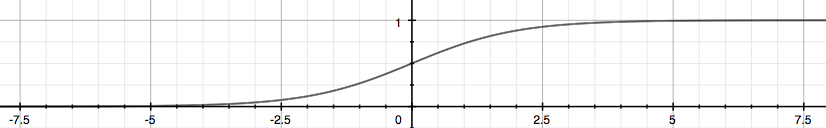
\includegraphics[scale=0.5]{W3_sigmoid}
\caption{Sigmoid Function}
\label{fig:W3_sigmoid}
\end{figure}

The function g(z), shown here, maps any real number to the (0, 1) interval, making it useful for transforming an arbitrary-valued function into a function better suited for classification. Try playing with interactive plot of sigmoid function: \href{https://www.desmos.com/calculator/bgontvxotm}{click here!}.

We start with our old hypothesis (linear regression), except that we want to restrict the range to 0 and 1. This is accomplished by plugging $\theta^T $ into the Logistic Function.

$h_\theta $ will give us the probability that our output is 1. For example, $h_\theta(x)=0.7$ gives us the probability of 70\% that our output is 1.

\begin{align*}
&h_\theta(x) = P(y=1 | x ; \theta) = 1 - P(y=0 | x ; \theta) \\ 
&P(y = 0 | x;\theta) + P(y = 1 | x ; \theta) = 1
\end{align*}

Our probability that our prediction is 0 is just the complement of our probability that it is 1 (e.g. if probability that it is 1 is 70\%, then the probability that it is 0 is 30\%).
\section{Decision Boundary}
In order to get our discrete 0 or 1 classification, we can translate the output of the hypothesis function as follows:
\begin{align*}
& h_\theta(x) \geq 0.5 \rightarrow y = 1 \\
& h_\theta(x) < 0.5 \rightarrow y = 0 \\
\end{align*}
The way our logistic function g behaves is that when its input is greater than or equal to zero, its output is greater than or equal to 0.5:
\begin{align*}
g(z) \geq 0.5 \\
\text{when } z \geq 0
\end{align*}
Remember:
\begin{align*}
z=0,  e^{0}=1 \Rightarrow  g(z)=1/2\\ 
z \to \infty, e^{-\infty} \to 0 \Rightarrow g(z)=1 \\ 
z \to -\infty, e^{\infty}\to \infty \Rightarrow g(z)=0 
\end{align*}

So if our input to g is $\theta^T$, then that means:
\begin{align*}
& h_\theta(x) = g(\theta^T x) \geq 0.5 \\
& \text{when} \; \theta^T x \geq 0
\end{align*}

From these statements we can now say:
\begin{align*}
& \theta^T x \geq 0 \Rightarrow y = 1 \\
& \theta^T x < 0 \Rightarrow y = 0 \\
\end{align*}

The {\bf decision boundary} is the line that separates the area where y = 0 and where y = 1. It is created by our hypothesis function.

Example:
\begin{align*}
& \theta = 
\begin{bmatrix}
5 \\ 
-1 \\ 
0
\end{bmatrix} \\ 
& y = 1 \; if \; 5 + (-1) x_1 + 0 x_2 \geq 0 \\ 
& 5 - x_1 \geq 0 \\ 
& - x_1 \geq -5 \\
& x_1 \leq 5 \\ 
\end{align*}

In this case, our decision boundary is a straight vertical line placed on the graph where $x_1 = 5$, and everything to the left of that denotes y = 1, while everything to the right denotes y = 0.

Again, the input to the sigmoid function g(z) (e.g. $\theta^T X$) doesn't need to be linear, and could be a function that describes a circle (e.g.$ z = \theta_0 + \theta_1 x_1^2 +\theta_2 x_2^2$) or any shape to fit our data.

\section{Cost Function}
We cannot use the same cost function that we use for linear regression because the Logistic Function will cause the output to be wavy, causing many local optima. In other words, it will not be a convex function.

Instead, our cost function for logistic regression looks like:
\begin{equation}
J(\theta) = \dfrac{1}{m} \sum_{i=1}^m \mathrm{Cost}(h_\theta(x^{(i)}),y^{(i)})
\end{equation}

\begin{align*}
\mathrm{Cost}(h_\theta(x),y) &= -\log(h_\theta(x)) \; \quad& \text{if y = 1} \\ 
\mathrm{Cost}(h_\theta(x),y) &= -\log(1-h_\theta(x)) \; \quad& \text{if y = 0}
\end{align*}

\begin{figure}[ht]
\center
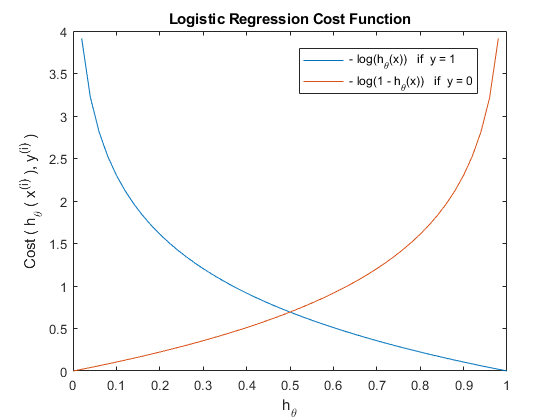
\includegraphics[scale=0.7]{W3_costlogistic}
\caption{Logistic Regression Cost Function}
\label{fig:W3_cost}
\end{figure}

The more our hypothesis is off from y, the larger the cost function output. If our hypothesis is equal to y, then our cost is 0:
\begin{align*}
& \mathrm{Cost}(h_\theta(x),y) = 0 \text{  if  } h_\theta(x) = y \\ 
& \mathrm{Cost}(h_\theta(x),y) \rightarrow \infty \text{  if  } y = 0 \; \mathrm{and} \; h_\theta(x) \rightarrow 1 \\ 
& \mathrm{Cost}(h_\theta(x),y) \rightarrow \infty \text{  if  } y = 1 \; \mathrm{and} \; h_\theta(x) \rightarrow 0 \\ 
\end{align*}
If our correct answer `y' is 0, then the cost function will be 0 if our hypothesis function also outputs 0. If our hypothesis approaches 1, then the cost function will approach infinity.

If our correct answer `y' is 1, then the cost function will be 0 if our hypothesis function outputs 1. If our hypothesis approaches 0, then the cost function will approach infinity.

Note that writing the cost function in this way guarantees that $J(\theta)$ is convex for logistic regression.

\section{Simplified Cost Function and Gradient Descent}
We can compress our cost function's two conditional cases into one case:

\begin{equation}
\mathrm{Cost}(h_\theta(x),y) = - y \; \log(h_\theta(x)) - (1 - y) \log(1 - h_\theta(x))
\end{equation}

Notice that when y is equal to 1, then the second term $(1-y)\log(1-h_\theta(x))$ will be zero and will not affect the result. If y is equal to 0, then the first term $-y \log(h_\theta(x))$ will be zero and will not affect the result.

We can fully write out our entire cost function as follows:

\begin{equation}
J(\theta) = - \frac{1}{m} \displaystyle \sum_{i=1}^m [y^{(i)}\log (h_\theta (x^{(i)})) + (1 - y^{(i)})\log (1 - h_\theta(x^{(i)}))]
\end{equation}

A vectorized implementation is:
\begin{align}
h &= g(X\theta)\\
J(\theta)  &= \frac{1}{m} \cdot \left(-y^{T}\log(h)-(1-y)^{T}\log(1-h)\right)
\end{align}

\subsection{Gradient Descent}
Remember that the general form of gradient descent is:
\begin{align*}
& Repeat \; \lbrace \\ 
& \; \theta_j := \theta_j - \alpha \dfrac{\partial}{\partial \theta_j}J(\theta) \\ 
& \rbrace
\end{align*}

We can work out the derivative part using calculus to get:

\begin{align*}
& Repeat \; \lbrace \\
& \; \theta_j := \theta_j - \frac{\alpha}{m} \sum_{i=1}^m (h_\theta(x^{(i)}) - y^{(i)}) x_j^{(i)} \\ & \rbrace
\end{align*}

Notice that this algorithm is identical to the one we used in linear regression. We still have to simultaneously update all values in theta.

A vectorized implementation is:
\[\theta := \theta - \frac{\alpha}{m} X^{T} (g(X \theta ) - \vec{y}) \]

\subsection{Partial derivative of Cost Function}

First calculate derivative of sigmoid function (it will be useful while finding partial derivative of $J(\theta)$

{\small
\begin{align*}
\sigma(x)'
&=\left(\frac{1}{1+e^{-x}}\right)'=\frac{-(1+e^{-x})'}{(1+e^{-x})^2}\\
&=\frac{-1'-(e^{-x})'}{(1+e^{-x})^2}=\frac{0-(-x)'(e^{-x})}{(1+e^{-x})^2}\\
&=\frac{-(-1)(e^{-x})}{(1+e^{-x})^2}=\frac{e^{-x}}{(1+e^{-x})^2} \\ 
&=\left(\frac{1}{1+e^{-x}}\right)\left(\frac{e^{-x}}{1+e^{-x}}\right)\\
&=\sigma(x)\left(\frac{+1-1 + e^{-x}}{1+e^{-x}}\right)\\
&=\sigma(x)\left(\frac{1 + e^{-x}}{1+e^{-x}} - \frac{1}{1+e^{-x}}\right)\\
&=\sigma(x)(1 - \sigma(x))
\end{align*}
}

Now we are ready to find out resulting partial derivative:
{\small
\begin{align*}
&\frac{\partial}{\partial \theta_j} J(\theta)= \\ 
&= \frac{\partial}{\partial \theta_j} \frac{-1}{m}\sum_{i=1}^m \left [ y^{(i)} log (h_\theta(x^{(i)})) + (1-y^{(i)}) log (1 - h_\theta(x^{(i)})) \right ] \\
&= - \frac{1}{m}\sum_{i=1}^m \left [     y^{(i)} \frac{\partial}{\partial \theta_j} log (h_\theta(x^{(i)}))   + (1-y^{(i)}) \frac{\partial}{\partial \theta_j} log (1 - h_\theta(x^{(i)}))\right ] \\
&= - \frac{1}{m}\sum_{i=1}^m \left [     \frac{y^{(i)} \frac{\partial}{\partial \theta_j} h_\theta(x^{(i)})}{h_\theta(x^{(i)})}   + \frac{(1-y^{(i)})\frac{\partial}{\partial \theta_j} (1 - h_\theta(x^{(i)}))}{1 - h_\theta(x^{(i)})}\right ] \\
&= - \frac{1}{m}\sum_{i=1}^m \left [     \frac{y^{(i)} \frac{\partial}{\partial \theta_j} \sigma(\theta^T x^{(i)})}{h_\theta(x^{(i)})}   + \frac{(1-y^{(i)})\frac{\partial}{\partial \theta_j} (1 - \sigma(\theta^T x^{(i)}))}{1 - h_\theta(x^{(i)})}\right ] \\
&= - \frac{1}{m}\sum_{i=1}^m \left [     \frac{y^{(i)} \sigma(\theta^T x^{(i)}) (1 - \sigma(\theta^T x^{(i)})) \frac{\partial}{\partial \theta_j} \theta^T x^{(i)}}{h_\theta(x^{(i)})}   + \frac{- (1-y^{(i)}) \sigma(\theta^T x^{(i)}) (1 - \sigma(\theta^T x^{(i)})) \frac{\partial}{\partial \theta_j} \theta^T x^{(i)}}{1 - h_\theta(x^{(i)})}\right ] \\
&= - \frac{1}{m}\sum_{i=1}^m \left [     \frac{y^{(i)} h_\theta(x^{(i)}) (1 - h_\theta(x^{(i)})) \frac{\partial}{\partial \theta_j} \theta^T x^{(i)}}{h_\theta(x^{(i)})}   - \frac{(1-y^{(i)}) h_\theta(x^{(i)}) (1 - h_\theta(x^{(i)})) \frac{\partial}{\partial \theta_j} \theta^T x^{(i)}}{1 - h_\theta(x^{(i)})}\right ] \\
&= - \frac{1}{m}\sum_{i=1}^m \left [     y^{(i)} (1 - h_\theta(x^{(i)})) x^{(i)}_j - (1-y^{(i)}) h_\theta(x^{(i)}) x^{(i)}_j\right ] \\
&= - \frac{1}{m}\sum_{i=1}^m \left [     y^{(i)} (1 - h_\theta(x^{(i)})) - (1-y^{(i)}) h_\theta(x^{(i)}) \right ] x^{(i)}_j \\
&= - \frac{1}{m}\sum_{i=1}^m \left [     y^{(i)} - y^{(i)} h_\theta(x^{(i)}) - h_\theta(x^{(i)}) + y^{(i)} h_\theta(x^{(i)}) \right ] x^{(i)}_j \\
&= - \frac{1}{m}\sum_{i=1}^m \left [ y^{(i)} - h_\theta(x^{(i)}) \right ] x^{(i)}_j  \\
&= \frac{1}{m}\sum_{i=1}^m \left [ h_\theta(x^{(i)}) - y^{(i)} \right ] x^{(i)}_j
\end{align*}
}

The vectorized version:
\begin{equation}
\nabla J(\theta) = \frac{1}{m} \cdot X^T \cdot \left(g\left(X\cdot\theta\right) - \vec{y}\right)
\end{equation}

\section{Advances Optimization}
\textbf{``Conjugate gradient"}, \textbf{``BFGS"}, and \textbf{``L-BFGS"} are more sophisticated, faster ways to optimize $\theta$ that can be used instead of gradient descent. A. Ng suggests not to write these more sophisticated algorithms yourself (unless you are an expert in numerical computing) but use the libraries instead, as they're already tested and highly optimized. Octave provides them.

We first need to provide a function that evaluates the following two functions for a given input value $\theta$:

\begin{align*}
J(\theta)\\
\frac{\partial}{\partial\theta_j}J(\theta)
\end{align*}

We can write a single function that returns both of these:

\begin{verbatim}
function [jVal, gradient] = costFunction(theta)
  jVal = [...code to compute J(theta)...];
  gradient = [...code to compute derivative of J(theta)...];
end
\end{verbatim}

Then we can use octave's \verb| fminunc()| optimization algorithm along with the \verb|optimset()| function that creates an object containing the options we want to send to \verb| fminunc()|. (Note: the value for MaxIter should be an integer, not a character string - errata in the video at 7:30)

\begin{verbatim}
options = optimset('GradObj', 'on', 'MaxIter', 100);
      initialTheta = zeros(2,1);
      [optTheta, functionVal, exitFlag] = fminunc(@costFunction, initialTheta, options);
\end{verbatim}

We give to the function \verb| fminunc()| our cost function, our initial vector of theta values, and the \textbf{options} object that we created beforehand.

\section{Multiclass Classification: One-vs-all}
Now we will approach the classification of data into more than two categories. Instead of $y = {0,1}$ we will expand our definition so that $y = {0,1...n}$.

In this case we divide our problem into n+1 (+1 because the index starts at 0) binary classification problems; in each one, we predict the probability that `y' is a member of one of our classes.

\begin{align*}
& y \in \lbrace0, 1 ... n\rbrace \\
& h_\theta^{(0)}(x) = P(y = 0 | x ; \theta) \\
& h_\theta^{(1)}(x) = P(y = 1 | x ; \theta) \\
& \cdots \\
& h_\theta^{(n)}(x) = P(y = n | x ; \theta) \\
& \mathrm{prediction} = \max_i( h_\theta ^{(i)}(x) )\\
\end{align*}

We are basically choosing one class and then lumping all the others into a single second class. We do this repeatedly, applying binary logistic regression to each case, and then use the hypothesis that returned the highest value as our prediction.

\section{ML: Regularization}
{\bf The Problem of Overfitting}
Regularization is designed to address the problem of overfitting.

High bias or underfitting is when the form of our hypothesis function h maps poorly to the trend of the data. It is usually caused by a function that is too simple or uses too few features. eg. if we take $h_\theta(x) = \theta_0 + \theta_1x_1 + \theta_2x_2$ then we are making an initial assumption that a linear model will fit the training data well and will be able to generalize but that may not be the case.

At the other extreme, overfitting or high variance is caused by a hypothesis function that fits the available data but does not generalize well to predict new data. It is usually caused by a complicated function that creates a lot of unnecessary curves and angles unrelated to the data.

This terminology is applied to both linear and logistic regression. There are two main options to address the issue of overfitting:

\begin{itemize}
  \item[1)] Reduce the number of features
  \begin{itemize}
  	\item[A)] Manually select which features to keep. 
  	\item[B)] Use a model selection algorithm (studied later in the course).
  \end{itemize}
  \item[2)] Regularization
  \begin{itemize}
  	\item[A)] Keep all the features, but reduce the parameters $\theta_j$
  	\item[B)] Regularization works well when we have a lot of slightly useful features.
  \end{itemize}  
\end{itemize}

\section{Cost Function}
f we have overfitting from our hypothesis function, we can reduce the weight that some of the terms in our function carry by increasing their cost.

Say we wanted to make the following function more quadratic:

$$\theta_0 + \theta_1x + \theta_2x^2 + \theta_3x^3 + \theta_4x^4$$

We'll want to eliminate the influence of $\theta_3x^3$ and $\theta_4x^4$. Without actually getting rid of these features or changing the form of our hypothesis, we can instead modify our \textbf{cost function}:
\begin{equation}
min_\theta\ \dfrac{1}{2m}\sum_{i=1}^m (h_\theta(x^{(i)}) - y^{(i)})^2 + 1000\cdot\theta_3^2 + 1000\cdot\theta_4^2
\end{equation}

We've added two extra terms at the end to inflate the cost of $\theta_3$ and $\theta_4$. Now, in order for the cost function to get close to zero, we will have to reduce the values of $\theta_3$ and $\theta_4$ to near zero. This will in turn greatly reduce the values of $\theta_3x^3$ and $\theta_4x^4$ in our hypothesis function.

We could also regularize all of our theta parameters in a single summation:

\begin{equation}
min_\theta\ \dfrac{1}{2m}\ \left[ \sum_{i=1}^m (h_\theta(x^{(i)}) - y^{(i)})^2 + \lambda\ \sum_{j=1}^n \theta_j^2 \right]
\end{equation}

The $\lambda$, or lambda, is \textbf{the regularization parameter}. It determines how much the costs of our theta parameters are inflated. You can visualize the effect of regularization in this \href{https://www.desmos.com/calculator/1hexc8ntqp}{interactive plot}

Using the above cost function with the extra summation, we can smooth the output of our hypothesis function to reduce overfitting. If lambda is chosen to be too large, it may smooth out the function too much and cause underfitting.

\section{Regularized Linear Regression}
We can apply regularization to both linear regression and logistic regression. We will approach linear regression first.

\subsection{Gradient Descent}
We will modify our gradient descent function to separate out $\theta_0$ from the rest of the parameters because we do not want to penalize $\theta_0$.
\begin{align*}
& \text{Repeat}\ \lbrace \\
& \ \ \ \ \theta_0 := \theta_0 - \alpha\ \frac{1}{m}\ \sum_{i=1}^m (h_\theta(x^{(i)}) - y^{(i)})x_0^{(i)} \\
& \ \ \ \ \theta_j := \theta_j - \alpha\ \left[ \left( \frac{1}{m}\ \sum_{i=1}^m (h_\theta(x^{(i)}) - y^{(i)})x_j^{(i)} \right) + \frac{\lambda}{m}\theta_j \right] &\ \ \ \ \ \ \ \ \ \ j \in \lbrace 1,2...n\rbrace\newline
& \rbrace
\end{align*}

The term $\frac{\lambda}{m}\theta_j$ performs our regularization.
With some manipulation our update rule can also be represented as:

\begin{equation}
\theta_j := \theta_j(1 - \alpha\frac{\lambda}{m}) - \alpha\frac{1}{m}\sum_{i=1}^m(h_\theta(x^{(i)}) - y^{(i)})x_j^{(i)}
\end{equation}

The first term in the above equation, $1 - \alpha\frac{\lambda}{m}$ will always be less than 1. Intuitively you can see it as reducing the value of $\theta_j$ by some amount on every update.

Notice that the second term is now exactly the same as it was before.

\subsection{Normal Equation}
Now let's approach regularization using the alternate method of the non-iterative normal equation.

To add in regularization, the equation is the same as our original, except that we add another term inside the parentheses:

\begin{align*}
& \theta = \left( X^TX + \lambda \cdot L \right)^{-1} X^Ty \\
& \text{where}\ \ L = 
\begin{bmatrix} 
0 & & & & \\ 
& 1 & & & \\ 
& & 1 & & \\ 
& & & \ddots & \\
& & & & 1 \\
\end{bmatrix}
\end{align*}

L is a matrix with 0 at the top left and 1's down the diagonal, with 0's everywhere else. It should have dimension $(n+1)\times(n+1)$. Intuitively, this is the identity matrix (though we are not including $x_0$), multiplied with a single real number $\lambda$.

Recall that if $m \leq n$, then $X^TX$ is non-invertible. However, when we add the term $\lambda \cdot L$, then $X^TX + \lambda \cdot L$ becomes invertible.
 
 \section{Regularized Logistic Regression}
 
\chapter{Week 4}
\section{ML: Neural Networks: Representation}
\subsection{Non-linear Hypothesis}
Performing linear regression with a complex set of data with many features is very unwieldy. Say you wanted to create a hypothesis from three (3) features that included all the quadratic terms:

\begin{align*}
&g(\theta_0 + \theta_1 x_1^2 + \theta_2x_1x_2+ \theta_3x_1x_3 \\
&+ \theta_4x_2^2 + \theta_5x_2x_3 \\
&+\theta_6x_3^2)
\end{align*}

That gives us 6 features. The exact way to calculate how many features for all polynomial terms is the combination function with repetition:

\href{http://www.mathsisfun.com/combinatorics/combinations-permutations.html}{Combinations and permutations} $\frac{(n+r-1)!}{r!(n-1)!}$.

In this case we are taking all two-element combinations of three features: $\frac{(3 + 2 - 1)!}{(2!\cdot (3-1)!)} = \frac{4!}{4} = 6 $.
(\textbf{Note}: you do not have to know these formulas, I just found helpful for understanding).

For 100 features, if we wanted to make the quadratic we would get $ \frac{(100 + 2 - 1)!}{(2\cdot (100-1)!)} = 5050 $ resulting new features.

We can approximate the growth of the number of new features we get with all quadratic terms with $\mathcal{O}(n^2/2)$. And if you wanted to include all cubic terms in your hypothesis, the features would grow asymptotically at $\mathcal{O}(n^3)$. These are very steep growths, so as the number of our features increase, the number of quadratic or cubic features increase very rapidly and becomes quickly impractical.

Example: let our training set be a collection of 50 x 50 pixel black-and-white photographs, and our goal will be to classify which ones are photos of cars. Our feature set size is then n = 2500 if we compare every pair of pixels.

Now let's say we need to make a quadratic hypothesis function. With quadratic features, our growth is $\mathcal{O}(n^2/2)$. So our total features will be about $2500^2 / 2 = 3125000 $, which is very impractical.

Neural networks offers an alternate way to perform machine learning when we have complex hypotheses with many features.

\section{Neurons and the Brain}

Neural networks are limited imitations of how our own brains work. They've had a big recent resurgence because of advances in computer hardware.

There is evidence that \textbf{the brain uses only one ``learning algorithm"} for all its different functions. Scientists have tried cutting (in an animal brain) the connection between the ears and the auditory cortex and rewiring the optical nerve with the auditory cortex to find that the auditory cortex literally learns to see.

This principle is called ``\textbf{neuroplasticity}" and has many examples and experimental evidence.

\section{Model Representation I}
Let's examine how we will represent a hypothesis function using neural networks.

At a very simple level, neurons are basically computational units that take input \textbf{dendrites} as electrical input (called ``\textbf{spikes}") that are channeled to outputs (\textbf{axons}).

In our model, our dendrites are like the input features $x_1\cdots x_n$, and the output is the result of our hypothesis function:

In this model our $x0$ input node is sometimes called the ``bias unit." It is always equal to 1.

In neural networks, we use the same logistic function as in classification: $\frac{1}{1 + e^{-\theta^Tx}} $. In neural networks however we sometimes call it a \textbf{sigmoid} (logistic) activation function.

Our ``theta" parameters are sometimes instead called \textbf{weights} in the neural networks model.

Visually, a simplistic representation looks like:
\[ [x_0x_1x_2]\rightarrow [\quad] \rightarrow h_\theta (x) \]

Our input nodes (layer 1) go into another node (layer 2), and are output as the hypothesis function.

The first layer is called the \textbf{input layer} and the final layer the \textbf{output layer}, which gives the final value computed on the hypothesis.

We can have intermediate layers of nodes between the input and output layers called the \textbf{hidden layer}.

We label these intermediate or \textbf{``hidden"} layer nodes $a^2_0 \cdots a^2_n $ and call them \textbf{activation units}.

\begin{align*}
& a_i^{(j)} = \text{``activation" of unit $i$ in layer $j$} \\
& \Theta^{(j)} = \text{matrix of weights controlling function mapping from layer $j$ to layer $j+1$}
\end{align*}

If we had one hidden layer, it would look visually something like:

\[ [x_0x_1x_2]\rightarrow [a_1^{(2)}a_2^{(2)}a_3^{(2)}] \rightarrow h_\theta (x) \]

The values for each \textbf{activation} nodes is obtained as follows:
\begin{align*}
a_1^{(2)} &= g(\Theta_{10}^{(1)}x_0 + \Theta_{11}^{(1)}x_1 + \Theta_{12}^{(1)}x_2 + \Theta_{13}^{(1)}x_3) \\
a_2^{(2)} &= g(\Theta_{20}^{(1)}x_0 + \Theta_{21}^{(1)}x_1 + \Theta_{22}^{(1)}x_2 + \Theta_{23}^{(1)}x_3) \\
a_3^{(2)} &= g(\Theta_{30}^{(1)}x_0 + \Theta_{31}^{(1)}x_1 + \Theta_{32}^{(1)}x_2 + \Theta_{33}^{(1)}x_3) \\ \\
h_\Theta(x) = a_1^{(3)} &= g(\Theta_{10}^{(2)}a_0^{(2)} + \Theta_{11}^{(2)}a_1^{(2)} + \Theta_{12}^{(2)}a_2^{(2)} + \Theta_{13}^{(2)}a_3^{(2)})
\end{align*}

This is saying that we compute our activation nodes by using a 3x4 matrix of parameters. We apply each row of the parameters to our inputs to obtain the value for one activation node. Our hypothesis output is the logistic function applied to the sum of the values of our activation nodes, which have been multiplied by yet another parameter matrix $\Theta^{(2)}$ containing the weights for our second layer of nodes.

Each layer gets its own matrix of weights, $\Theta^{(j)}$.

The dimensions of these matrices of weights is determined as follows:
\begin{quote}
If network has $s_j$ units in layer $j$  and $s_{j+1}$ units in layer $j+1$, then $\Theta_0^{j}$ will be of dimension $s_{s+j}\times(s_j+1)$
\end{quote}

The +1 comes from the addition in $\Theta^{(j)}$ of the \textbf{bias nodes}, $x_0$ and $\Theta_0^{(j)}$. In other words the output nodes will not include the bias nodes while the inputs will.

\textbf{Example}: layer 1 has 2 input nodes and layer 2 has 4 activation nodes. Dimension of $\Theta^{(1)}$ is going to be $4\times 3$ where $s_j = 2$ and $s_{j+1} = 4$, so: $$s_{j+1} \times (s_j + 1) = 4 \times 3$$

\section{Model Representation II}
In this section we'll do a vectorized implementation of the above functions. We're going to define a new variable $z_k^{(j)}$ that encompasses the parameters inside our g function. In our previous example if we replaced the variable z for all the parameters we would get:

\begin{align*}
a_1^{(2)} = g(z_1^{(2)}) \\
a_2^{(2)} = g(z_2^{(2)}) \\ 
a_3^{(2)} = g(z_3^{(2)})
\end{align*}
In other words, for layer j=2 and node k, the variable z will be:
\[
z_k^{(2)} = \Theta_{k,0}^{(1)}x_0 + \Theta_{k,1}^{(1)}x_1 + \cdots + \Theta_{k,n}^{(1)}x_n
\]

The vector representation of $x$ and $z^{j}$ is:
\begin{align*}
x = 
\begin{bmatrix}
x_0 \\ 
x_1 \\
\cdots \\ 
x_n
\end{bmatrix} 
&z^{(j)} = 
\begin{bmatrix}
z_1^{(j)} \\
z_2^{(j)} \\
\cdots \\ 
z_n^{(j)}
\end{bmatrix}
\end{align*}

Setting $x = a^{(1)}$, we can rewrite the equation as:

\[z^{(j)} = \Theta^{(j-1)} a^{(j-1)} \]

We are multiplying our matrix $\Theta^{(j-1)}$ with dimensions $s_j\times (n+1)$ (where $s_j$ is the number of our activation nodes) by our vector $a^{(j-1)}$ with height $(n+1)$. This gives us our vector $z^{(j)}$ with height $s_j$.

Now we can get a vector of our activation nodes for layer j as follows:

$$a^{(j)} = g(z^{(j)})$$

Where our function g can be applied element-wise to our vector $z^{(j)}$.

We can then add a bias unit (equal to 1) to layer j after we have computed $a^{(j)}$. This will be element $a_0^{(j)}$ and will be equal to 1.

To compute our final hypothesis, let's first compute another z vector:

$$ z^{(j+1)} = \Theta^{(j)}a^{(j)} $$


We get this final z vector by multiplying the next theta matrix after $\Theta^{(j-1)}$ with the values of all the activation nodes we just got.

This last theta matrix $\Theta^{(j)}$ will have only one row so that our result is a single number.

We then get our final result with:

\begin{equation}
h_\theta (x) = a^{(j+1)} = g(z^{(j+1)})
\end{equation}

Notice that in this \textbf{last step}, between layer j and layer j+1, we are doing \textbf{exactly the same thing} as we did in logistic regression.

Adding all these intermediate layers in neural networks allows us to more elegantly produce interesting and more complex non-linear hypotheses.
\section{Examples and Intuitions I}
A simple example of applying neural networks is by predicting $x_1$ AND $x_2$, which is the logical `\textbf{and}' operator and is only true if both $x_1$ and $x_2$ are 1.

The graph of our functions will look like:

\begin{align*}
\begin{bmatrix}
x_0 \\ 
x_1 \\ 
x_2
\end{bmatrix} 
\rightarrow
\begin{bmatrix}
g(z^{(2)})
\end{bmatrix} 
\rightarrow 
h_\Theta(x)
\end{align*}
Remember that $x_0$ is our bias variable and is always 1.

Let's set our first theta matrix as:

\begin{equation*}
\Theta^{(1)} = [-30\quad20\quad20]
\end{equation*}

This will cause the output of our hypothesis to only be positive if both $x_1$ and $x_2$ are 1. In other words:

\begin{align*}
& h_\Theta(x) = g(-30 + 20x_1 + 20x_2) \\ \\ 
& x_1 = 0 \ \ and \ \ x_2 = 0 \ \ then \ \ g(-30) \approx 0 \\ 
& x_1 = 0 \ \ and \ \ x_2 = 1 \ \ then \ \ g(-10) \approx 0 \\
& x_1 = 1 \ \ and \ \ x_2 = 0 \ \ then \ \ g(-10) \approx 0 \\ 
& x_1 = 1 \ \ and \ \ x_2 = 1 \ \ then \ \ g(10) \approx 1
\end{align*}
So we have constructed one of the fundamental operations in computers by using a small neural network rather than using an actual \textbf{AND} gate. Neural networks can also be used to simulate all the other logical gates.
\section{Examples and Intuitions II}
The $\Theta^{(1)}$ matrices for \textbf{AND}, \textbf{NOR} and \textbf{OR} are:
\begin{align*}
AND:\quad \Theta^{(1)} &= \begin{bmatrix}-30 & 20 & 20\end{bmatrix} \\ 
NOR:\quad \Theta^{(1)} &= \begin{bmatrix}10 & -20 & -20\end{bmatrix} \\
OR:\quad\Theta^{(1)} &= \begin{bmatrix}-10 & 20 & 20\end{bmatrix} \\
\end{align*}

We can combine these to get the \textbf{XNOR} logical operator (which gives 1 if $x_1x$ and $x_2$ are both 0 or both 1).
\begin{align*}
\begin{bmatrix}x_0 \\ 
x_1 \\ 
x_2
\end{bmatrix} 
\rightarrow
\begin{bmatrix}
a_1^{(2)} \\ 
a_2^{(2)} 
\end{bmatrix} 
\rightarrow
\begin{bmatrix}
a^{(3)}
\end{bmatrix} 
\rightarrow 
h_\Theta(x)
\end{align*}
For the transition between the first and second layer, we'll use a $\Theta^{(1)}$ matrix that combines the values for \textbf{AND} and \textbf{NOR}:
\begin{equation*}
\Theta^{(1)} = [-30\quad 20 \quad 2010 \quad -20 \quad -20]
\end{equation*}

For the transition between second and third layer, we'll use a $\Theta^{(2)}$ matrix that combines the values for \textbf{OR}:
\begin{equation*}
\Theta^{(1)} = [-30\quad 20 \quad 2010 \quad -20 \quad -20]
\end{equation*}

\begin{equation*}
\Theta^{(1)} = [-10\quad 20 \quad 20]
\end{equation*}

Let's write out the values for all our nodes:
\begin{align*}
& a^{(2)} = g(\Theta^{(1)} \cdot x) \\
& a^{(3)} = g(\Theta^{(2)} \cdot a^{(2)}) \\
& h_\Theta(x) = a^{(3)}
\end{align*}
\section{Multiclass Classification}

To classify data into multiple classes, we let our hypothesis function return a vector of values. Say we wanted to classify our data into one of four final resulting classes:

\begin{align*}
\begin{bmatrix} x_0 \\ x_1 \\ x_2 \\ \cdots \\ x_n \end{bmatrix} 
\rightarrow
\begin{bmatrix} a_0^{(2)} \\ a_1^{(2)} \\ a_2^{(2)} \\ \cdots \\ a_n^{(2)} \end{bmatrix} 
\rightarrow
\begin{bmatrix} a_0^{(3)} \\ a_1^{(3)} \\ a_2^{(3)} \\ \cdots \\ a_n^{(3)} \end{bmatrix} 
\rightarrow  \cdots \rightarrow
\begin{bmatrix} h_\Theta(x)_1 \\ h_\Theta(x)_2 \\ h_\Theta(x)_3 \\ h_\Theta(x)_4 \end{bmatrix} 
\rightarrow
\end{align*}

Our final layer of nodes, when multiplied by its theta matrix, will result in another vector, on which we will apply the g() logistic function to get a vector of hypothesis values.

Our resulting hypothesis for one set of inputs may look like:

$$
h_\Theta(x) = [0010]
$$

In which case our resulting class is the third one down, or $h_\Theta(x)_3$.

We can define our set of resulting classes as y:

\begin{equation*}
y^{(i)}= 
\begin{bmatrix}1\\0\\0\\0 \end{bmatrix},
\begin{bmatrix}0\\1\\0\\0 \end{bmatrix},
\begin{bmatrix}0\\0\\1\\0 \end{bmatrix},
\begin{bmatrix}0\\0\\0\\1 \end{bmatrix}
\end{equation*}

Our final value of our hypothesis for a set of inputs will be one of the elements in y.


\chapter{Week 5}
\section{Neural Networks Learning}
Let's first define a few variables that we will need to use:
\begin{itemize}
	\item[A)] L= total number of layers in the network
	\item[B)] $s_1$ number of units(not including bias unit) in layer 1
	\item[C)] K=number of outputs units/classes
\end{itemize}
Recall that the cost function for regularized logistic regression was:
\begin{equation}
J(\theta) = - \frac{1}{m} \sum_{i=1}^m \large[ y^{(i)}\ \log (h_\theta (x^{(i)})) + (1 - y^{(i)})\ \log (1 - h_\theta(x^{(i)}))\large] + \frac{\lambda}{2m}\sum_{j=1}^n \theta_j^2
\end{equation}
For neural  networks, it is going to bee slightly more complicated:

\chapter{Bonus: Tutorial}
\section{How to classify your own images of digits}
This tutorial will guide you on how to use the classifier provided in exercise 3 to classify you own images like figure \ref{fig:w5_imgclass}:

\begin{figure}[ht]
\center
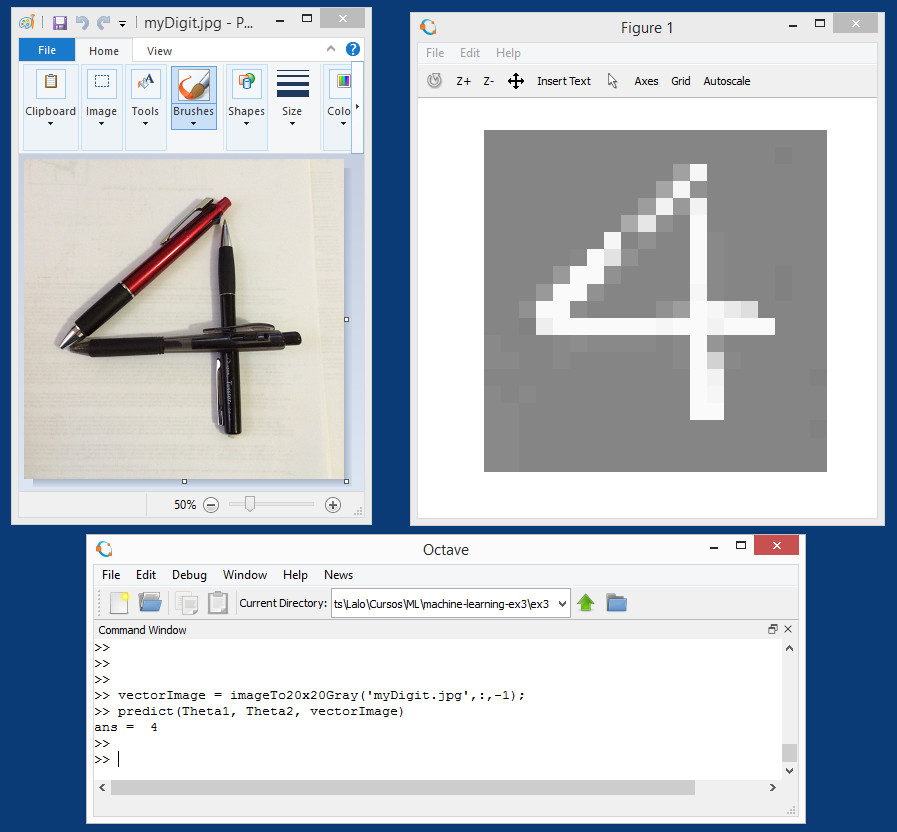
\includegraphics[scale=0.3]{W5_imgclass}
\caption{Image classifier}
\label{fig:w5_imgclass}
\end{figure}
It will also explain how the images are converted thru several formats to be processed and displayed.
\section{Introduction}
The classifier provided expects 20 x 20 pixels black and white images converted in a row vector of 400 real numbers like this:
\begin{verbatim}
[ 0.14532, 0.12876, ...]
\end{verbatim}
Each pixel is represented by a real number between -1.0 to 1.0, meaning -1.0 equal black and 1.0 equal white (any number in between is a shade of gray, and number 0.0 is exactly the middle gray).
\section{.jpg and color RGB images}
The most common image format that can be read by Octave is .jpg using function that outputs a three-dimensional matrix of integer numbers from 0 to 255, representing the height x width x 3 integers as indexes of a color map for each pixel (explaining color maps is beyond scope).

\begin{verbatim}
Image3DmatrixRGB = imread("myOwnPhoto.jpg");
\end{verbatim}

\section{Convert to Black \& White}
A common way to convert color images to black \& white, is to convert them to a YIQ standard and keep only the Y component that represents the luma information (black \& white). I and Q represent the chrominance information (color).Octave has a function \verb|rgb2ntsc()| that outputs a similar three-dimensional matrix but of real numbers from -1.0 to 1.0, representing the height x width x 3 (Y luma, I in-phase, Q quadrature) intensity for each pixel.
\begin{verbatim}
Image3DmatrixYIQ = rgb2ntsc(MyImageRGB);
\end{verbatim}
To obtain the Black \& White component just discard the I and Q matrices. This leaves a two-dimensional matrix of real numbers from -1.0 to 1.0 representing the height x width pixels black \& white values.
\begin{verbatim}
Image2DmatrixBW = Image3DmatrixYIQ(:,:,1);
\end{verbatim}
\section{Cropping to square image}
It is useful to crop the original image to be as square as possible. The way to crop a matrix is by selecting an area inside the original B\&W image and copy it to a new matrix. This is done by selecting the rows and columns that define the area. In other words, it is copying a rectangular subset of the matrix like this:
\begin{verbatim}
croppedImage = Image2DmatrixBW(origen1:size1, origin2:size2);
\end{verbatim}
Cropping does not have to be all the way to a square. \textbf{It could be cropping just a percentage of the way to a square} so you can leave more of the image intact. The next step of scaling will take care of streaching the image to fit a square.
\section{Scaling to 20 x 20 pixels}
The classifier provided was trained with 20 x 20 pixels images so we need to scale our photos to meet. It may cause distortion depending on the height and width ratio of the cropped original photo. There are many ways to scale a photo but we are going to use the simplest one. We lay a scaled grid of 20 x 20 over the original photo and take a sample pixel on the center of each grid. To lay a scaled grid, we compute two vectors of 20 indexes each evenly spaced on the original size of the image. One for the height and one for the width of the image. For example, in an image of 320 x 200 pixels will produce to vectors like
\begin{verbatim}
[9    25    41    57    73 ... 313] % 20 indexes

[6    16    26    36    46 ... 196] % 20 indexes
\end{verbatim}
Copy the value of each pixel located by the grid of these indexes to a new matrix. Ending up with a matrix of 20 x 20 real numbers.
\section{Black \& White to Gray \& White}
The classifier provided was trained with images of white digits over gray background. Specifically, the 20 x 20 matrix of real numbers ONLY range from 0.0 to 1.0 instead of the complete black \& white range of -1.0 to 1.0, this means that we have to normalize our photos to a range 0.0 to 1.0 for this classifier to work. But also, we invert the black and white colors because is easier to ``draw" black over white on our photos and we need to get white digits. So in short, we \textbf{invert black and white} and stretch \textbf{black to gray}.
\section{Rotation of image}
Some times our photos are automatically rotated like in our cellphone phones. The classifier provided can not recognize rotated images so we may need to rotate it back sometimes. This can be done with an Octave function \verb|rot90()| like this.
\begin{verbatim}
ImageAligned = rot90(Image, rotationStep);
\end{verbatim}
Where \verb|rotationStep| is an integer: -1 mean rotate 90 degrees CCW and 1 mean rotate 90 degrees CW.
\section{Approach}
\begin{enumerate}
	\item The approach is to have a function that converts our photo to the format the classifier is expecting. As if it was just a sample from the training data set.
	\item Use the classifier to predict the digit in the converted image.
\end{enumerate}
\section{Code step by step}
Define the function name, the output variable and three parameters, one for the filename of our photo, one optional cropping percentage (if not provided will default to zero, meaning no cropping) and the last optional rotation of the image (if not provided will default to cero, meaning no rotation).
\begin{verbatim}
function vectorImage = 
	imageTo20x20Gray(fileName, cropPercentage=0, rotStep=0)
\end{verbatim}
Read the file as a RGB image and convert it to Black \& White 2D matrix (see the introduction).
\begin{lstlisting}[language=Octave]
% Read as RGB image
Image3DmatrixRGB = imread(fileName);
% Convert to NTSC image (YIQ)
Image3DmatrixYIQ = rgb2ntsc(Image3DmatrixRGB );
% Convert to grays keeping only luminance (Y)
%        ...and discard chrominance (IQ)
Image2DmatrixBW  = Image3DmatrixYIQ(:,:,1);
\end{lstlisting}
Establish the final size of the cropped image.

\begin{verbatim}
% Get the size of your image
oldSize = size(Image2DmatrixBW);
% Obtain crop size toward centered square (cropDelta)
% ...will be zero for the already minimum dimension
% ...and if the cropPercentage is zero, 
% ...both dimensions are zero
% ...meaning that the original image will go intact to croppedImage
cropDelta = floor((oldSize - min(oldSize)) .* (cropPercentage/100));
% Compute the desired final pixel size for the original image
finalSize = oldSize - cropDelta;
\end{verbatim}

Obtain the origin and amount of the columns and rows to be copied to the cropped image.
\begin{verbatim}
% Compute each dimension origin for croping
cropOrigin = floor(cropDelta / 2) + 1;
% Compute each dimension copying size
copySize = cropOrigin + finalSize - 1;
% Copy just the desired cropped image from the original B&W image
croppedImage = Image2DmatrixBW( ...
                    cropOrigin(1):copySize(1), cropOrigin(2):copySize(2));
\end{verbatim}
Compute the scale and compute back the new size. This last step is extra. It is computed back so the code keeps general for future modification of the classifier size. For example: if changed from 20 x 20 pixels to 30 x 30. Then the we only need to change the line of code where the scale is computed.
\begin{verbatim}
% Resolution scale factors: [rows cols]
scale = [20 20] ./ finalSize;
% Compute back the new image size (extra step to keep code general)
newSize = max(floor(scale .* finalSize),1); 
\end{verbatim}
Compute two sets of 20 indexes evenly spaced. One over the original height and one over the original width of the image.

\begin{verbatim}
% Compute a re-sampled set of indices:
rowIndex = min(round(((1:newSize(1))-0.5)./scale(1)+0.5), finalSize(1));
colIndex = min(round(((1:newSize(2))-0.5)./scale(2)+0.5), finalSize(2));
\end{verbatim}
Copy just the indexed values from old image to get new image of 20 x 20 real numbers. This is called ``sampling" because it copies just a sample pixel indexed by a grid. All the sample pixels make the new image.

\begin{verbatim}
% Copy just the indexed values from old image to get new image
newImage = croppedImage(rowIndex,colIndex,:);
\end{verbatim}
Rotate the matrix using the \verb|rot90()| function with the rotStep parameter: -1 is CCW, 0 is no rotate, 1 is CW.
\begin{verbatim}
% Rotate if needed: -1 is CCW, 0 is no rotate, 1 is CW
newAlignedImage = rot90(newImage, rotStep);
\end{verbatim}
Invert black and white because it is easier to draw black digits over white background in our photos but the classifier needs white digits.
\begin{verbatim}
% Invert black and white
invertedImage = - newAlignedImage;
\end{verbatim}
Find the min and max gray values in the image and compute the total value range in preparation for normalization.
\begin{verbatim}
% Find min and max grays values in the image
maxValue = max(invertedImage(:));
minValue = min(invertedImage(:));
% Compute the value range of actual grays
delta = maxValue - minValue;
\end{verbatim}
Do normalization so all values end up between 0.0 and 1.0 because this particular classifier do not perform well with negative numbers.
\begin{verbatim}
% Normalize grays between 0 and 1
normImage = (invertedImage - minValue) / delta;
\end{verbatim}
Add some contrast to the image. The multiplication factor is the contrast control, you can increase it if desired to obtain sharper contrast (contrast only between gray and white, black was already removed in normalization).
\begin{verbatim}
% Add contrast. Multiplication factor is contrast control.
contrastedImage = sigmoid((normImage -0.5) * 5);
\end{verbatim}
Show the image specifying the black \& white range [-1 1] to avoid automatic ranging using the image range values of gray to white. Showing the photo with different range, does not affect the values in the output matrix, so do not affect the classifier. It is only as a visual feedback for the user.
\begin{verbatim}
% Show image as seen by the classifier
imshow(contrastedImage, [-1, 1] );
\end{verbatim}
Finally, output the matrix as a unrolled vector to be compatible with the classifier.

\begin{verbatim}
% Output the matrix as a unrolled vector
vectorImage = reshape(normImage, 1, newSize(1) * newSize(2));
\end{verbatim}
End function.

\verb|end;|

\section{Usage examples}
\subsection{Single photo}
\begin{itemize}
\item Photo file in myDigit.jpg
\item Cropping 60\% of the way to square photo
\item No \verb|rotationvectorImage| = \verb|imageTo20x20Gray('myDigit.jpg',60);|\\\verb| predict(Theta1, Theta2, vectorImage)|
\item Photo file in myDigit.jpg
\item No cropping
\item CCW rotationvectorImage = \verb|imageTo20x20Gray('myDigit.jpg',:,-1);|\\\verb| predict(Theta1, Theta2, vectorImage)|
\end{itemize}
\subsection{Multiple photos}
\begin{itemize}
\item Photo files in myFirstDigit.jpg, mySecondDigit.jpg
\item First crop to square and second 25\% of the way to square photo
\item First no rotation and second CW \\
\verb|rotationvectorImage(1,:)| = \verb|imageTo20x20Gray('myFirstDigit.jpg',100);|\\
\verb| vectorImage(2,:)| = \verb|imageTo20x20Gray('mySecondDigit.jpg',25,1);|\\\verb| predict(Theta1, Theta2, vectorImage)|
\end{itemize}

\subsection{Tips}
\begin{itemize}
\item JPG photos of black numbers over white background
\item Preferred square photos but not required
\item Rotate as needed because the classifier can only work with vertical digits
\item Leave background space around digit. Al least 2 pixels when seen at 20 x 20 resolution. This means that the classifier only really works in a 16 x 16 area.
\item Play changing the contrast multipier to 10 (or more).
\end{itemize}
\section{Complete code (just copy and paste)}
\begin{Verbatim}[fontsize=\small]
function vectorImage = imageTo20x20Gray(fileName, cropPercentage=0, rotStep=0)
%IMAGETO20X20GRAY display reduced image and converts for digit classification
%
% Sample usage: 
%       imageTo20x20Gray('myDigit.jpg', 100, -1);
%
%       First parameter: Image file name
%             Could be bigger than 20 x 20 px, it will
%             be resized to 20 x 20. Better if used with
%             square images but not required.
% 
%       Second parameter: cropPercentage (any number between 0 and 100)
%             0  0% will be cropped (optional, no needed for square images)
%            50  50% of available croping will be cropped
%           100  crop all the way to square image (for rectangular images)
% 
%       Third parameter: rotStep
%            -1  rotate image 90 degrees CCW
%             0  do not rotate (optional)
%             1  rotate image 90 degrees CW
%
% (Thanks to Edwin Frühwirth for parts of this code)
% Read as RGB image
Image3DmatrixRGB = imread(fileName);
% Convert to NTSC image (YIQ)
Image3DmatrixYIQ = rgb2ntsc(Image3DmatrixRGB );
% Convert to grays keeping only luminance (Y) and discard chrominance (IQ)
Image2DmatrixBW  = Image3DmatrixYIQ(:,:,1);
% Get the size of your image
oldSize = size(Image2DmatrixBW);
% Obtain crop size toward centered square (cropDelta)
% ...will be zero for the already minimum dimension
% ...and if the cropPercentage is zero, 
% ...both dimensions are zero
% ...meaning that the original image will go intact to croppedImage
cropDelta = floor((oldSize - min(oldSize)) .* (cropPercentage/100));
% Compute the desired final pixel size for the original image
finalSize = oldSize - cropDelta;
% Compute each dimension origin for croping
cropOrigin = floor(cropDelta / 2) + 1;
% Compute each dimension copying size
copySize = cropOrigin + finalSize - 1;
% Copy just the desired cropped image from the original B&W image
croppedImage = Image2DmatrixBW( ...
                    cropOrigin(1):copySize(1), cropOrigin(2):copySize(2));
% Resolution scale factors: [rows cols]
scale = [20 20] ./ finalSize;
% Compute back the new image size (extra step to keep code general)
newSize = max(floor(scale .* finalSize),1); 
% Compute a re-sampled set of indices:
rowIndex = min(round(((1:newSize(1))-0.5)./scale(1)+0.5), finalSize(1));
colIndex = min(round(((1:newSize(2))-0.5)./scale(2)+0.5), finalSize(2));
% Copy just the indexed values from old image to get new image
newImage = croppedImage(rowIndex,colIndex,:);
% Rotate if needed: -1 is CCW, 0 is no rotate, 1 is CW
newAlignedImage = rot90(newImage, rotStep);
% Invert black and white
invertedImage = - newAlignedImage;
% Find min and max grays values in the image
maxValue = max(invertedImage(:));
minValue = min(invertedImage(:));
% Compute the value range of actual grays
delta = maxValue - minValue;
% Normalize grays between 0 and 1
normImage = (invertedImage - minValue) / delta;
% Add contrast. Multiplication factor is contrast control.
contrastedImage = sigmoid((normImage -0.5) * 5);
% Show image as seen by the classifier
imshow(contrastedImage, [-1, 1] );
% Output the matrix as a unrolled vector
vectorImage = reshape(contrastedImage, 1, newSize(1)*newSize(2));
end
\end{Verbatim}
\section{Photo Gallery}
\begin{figure}[ht]
     \centering
     \begin{subfigure}[b]{0.47\textwidth}
         \centering
         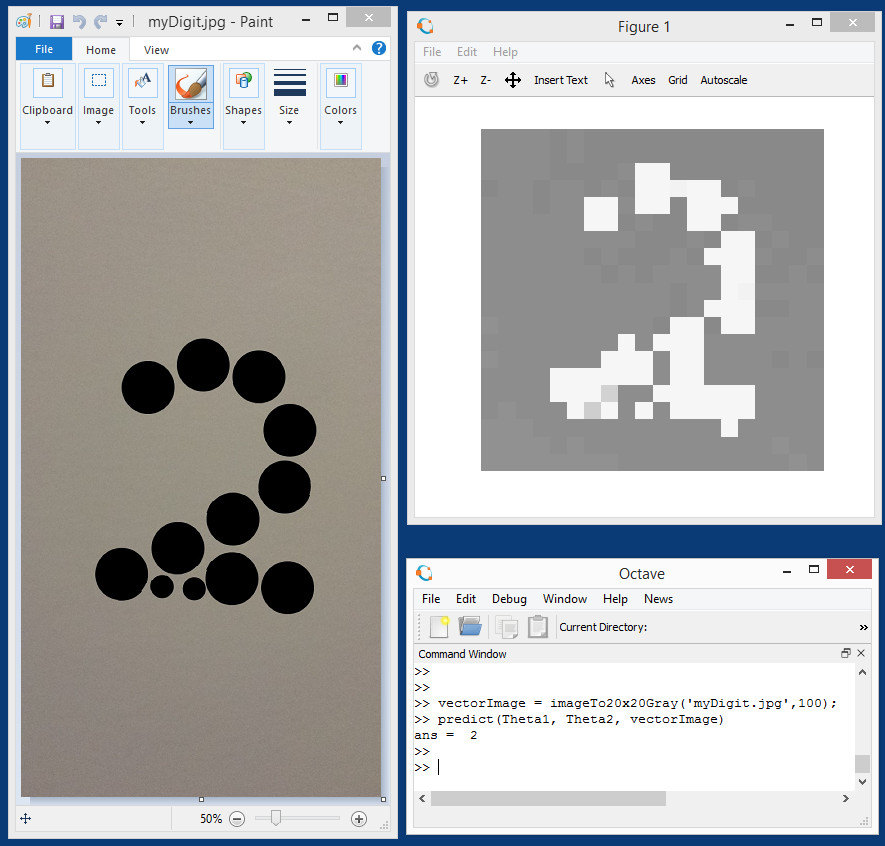
\includegraphics[width=\textwidth]{W5_a}
         \caption{Digit 2}
         \label{fig:W5_a}
     \end{subfigure}
     \hfill
     \begin{subfigure}[b]{0.47\textwidth}
         \centering
         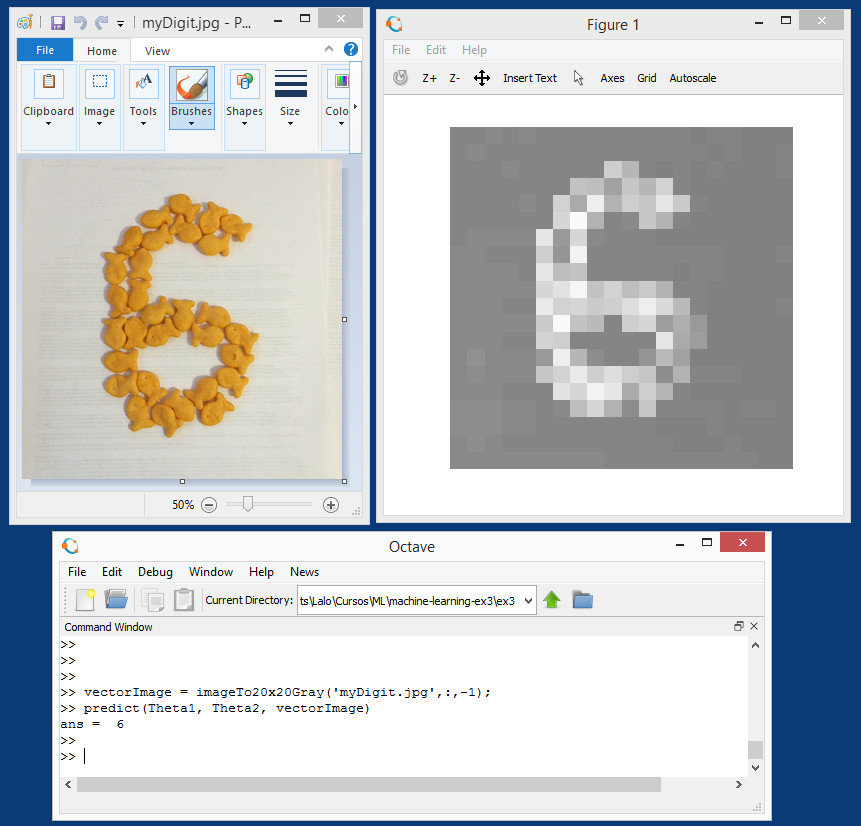
\includegraphics[width=\textwidth]{W5_b}
         \caption{Digit 6}
         \label{fig:W5_b}
     \end{subfigure}
     \hfill
     \begin{subfigure}[b]{0.47\textwidth}
         \centering
         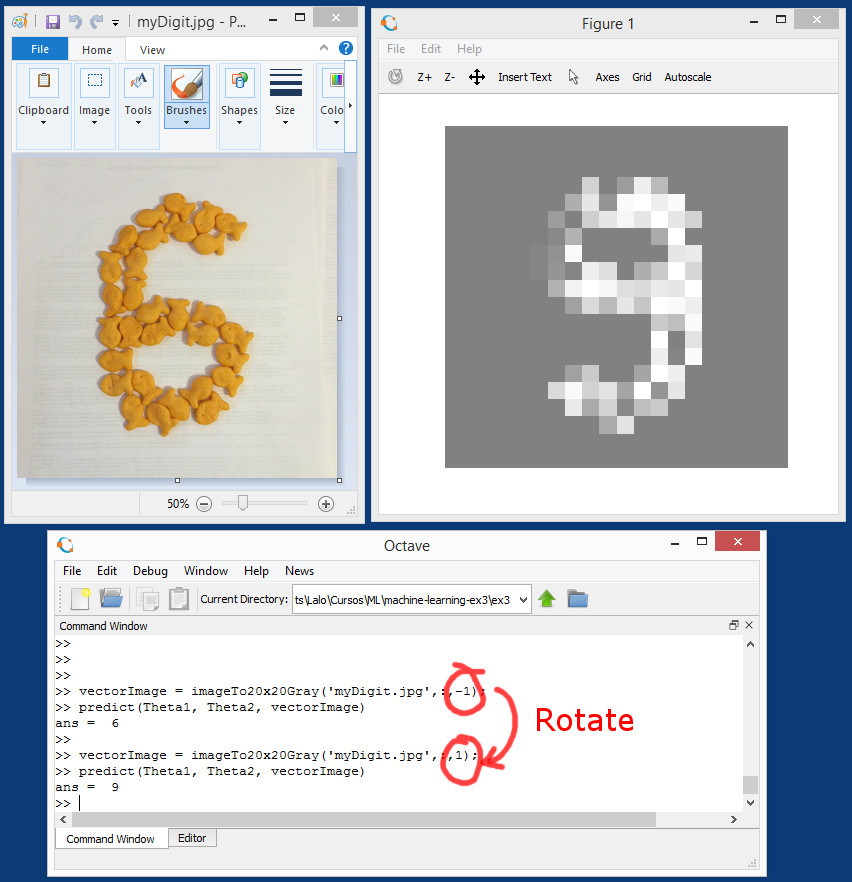
\includegraphics[width=\textwidth]{W5_c}
         \caption{Digit 9}
         \label{fig:W5_c}
     \end{subfigure}
     \hfill
     \begin{subfigure}[b]{0.47\textwidth}
         \centering
         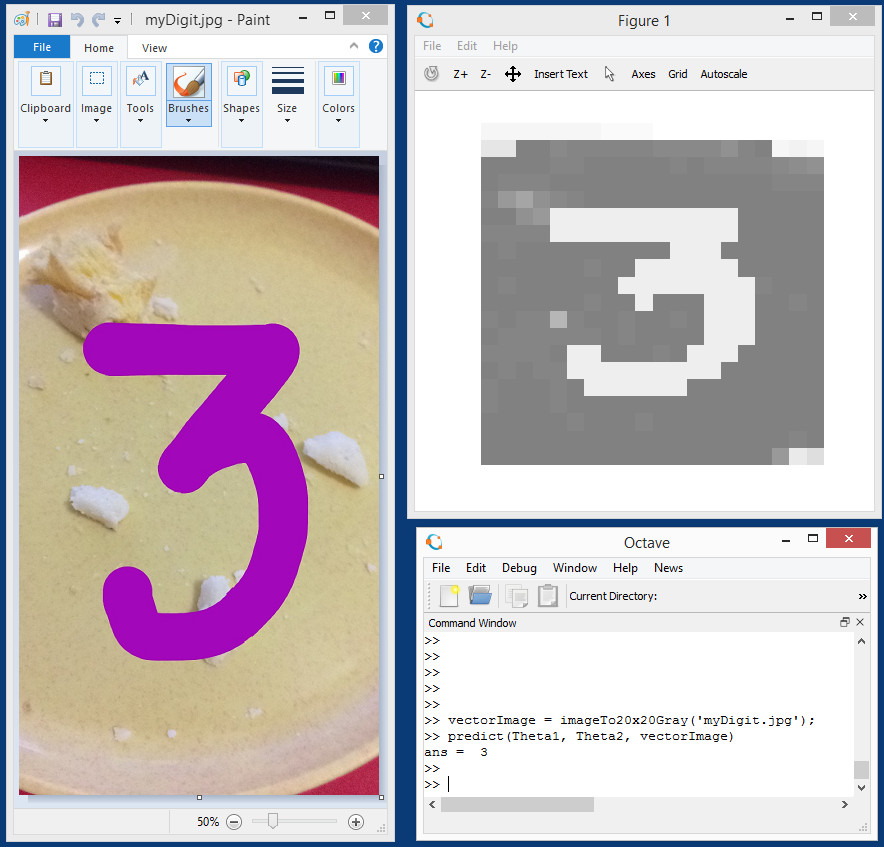
\includegraphics[width=\textwidth]{W5_d}
         \caption{Digit 3}
         \label{fig:W5_d}
     \end{subfigure}
        \caption{Photo Gallery}
        \label{fig:W5_gallery}
\end{figure}
Digit 6 inverted is digit 9 (figure \ref{fig:W5_c}). This is the same photo of a six but rotated. Also, changed the contrast multiplier from 5 to 20. You can note that the gray background is smoother.

\section{The Problem of Overfitting}
Consider the problem of predicting y from $x \in R$. The leftmost figure \ref{fig:w3_overfit} shows the result of fitting a $y=\theta_0 + \theta_1 x$ to a dataset. We see that the data doesn't really lie on straight line, and so the fit is not very good.
\begin{figure}[ht]
\center
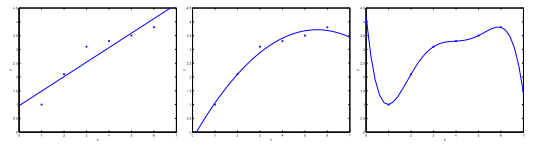
\includegraphics[scale=0.7]{W3_overfitting}
\caption{The Problem of Overfitting}
\label{fig:w3_overfit}
\end{figure}

Instead, if we had added an extra feature $x^2$, and fit $y = \theta_0 + \theta_1x + \theta_2x^2$, then we obtain a slightly better fit to the data (See middle figure). Naively, it might seem that the more features we add, the better. However, there is also a danger in adding too many features: The rightmost figure is the result of fitting a $5^{th}$ order polynomial $y = \sum_{j=0} ^5 \theta_j$. We see that even though the fitted curve passes through the data perfectly, we would not expect this to be a very good predictor of, say, housing prices (y) for different living areas (x). Without formally defining what these terms mean, we'll say the figure on the left shows an instance of {\bf underfitting}-in which the data clearly shows structure not captured by the model-and the figure on the right is an example of {\bf overfitting}.

Underfitting, or high bias, is when the form of our hypothesis function h maps poorly to the trend of the data. It is usually caused by a function that is too simple or uses too few features. At the other extreme, overfitting, or high variance, is caused by a hypothesis function that fits the available data but does not generalize well to predict new data. It is usually caused by a complicated function that creates a lot of unnecessary curves and angles unrelated to the data.

This terminology is applied to both linear and logistic regression. There are two main options to address the issue of overfitting:
\begin{itemize}
	\item[$1)$] Reduce the number of features:
	\item	\quad Manually select which features to keep.
	\item	\quad Use a model selection algorithm (studied later in the course).
	\item[$2)$] Regularization
	\item	\quad Keep all the features, but reduce the magnitude of parameters $\theta_j$
	\item	\quad Regularization works well when we have a lot of slightly useful features.
\end{itemize}
\chapter{Week 6}
\section{ML:Advice for Applying Machine Learning}
\subsection{Deciding what to do next}
Errors in your predictions can be troubleshooted by:
\begin{itemize}
	\item Getting more training examples
	\item Trying smaller sets of values
	\item Trying additional features
	\item Trying polynomial features
	\item Increasing ore decreasing $\lambda$
\end{itemize}
Don't just pick one of these avenues at random. We'll explore diagnostic techniques for choosing one of the above solutions in the following sections.
\section{Evaluating a Hypothesis}
A hypothesis may have low error for the training examples but still be inaccurate (because of overfitting).

With a given dataset of training examples, we can split up the data into two sets: a \textbf{training set} and a \textbf{test set}.

The new procedure using these two sets is then:

\begin{enumerate}
	\item Learn $\Theta$ and minimize $J_{train}(\Theta)$ using the training set.
	\item Compute the test set error $J_{test}(\Theta)$
\end{enumerate}
\subsection{The test set error}
\begin{enumerate}
\item For linear regression
\[J_{test}(\Theta) = \dfrac{1}{2m_{test}} \sum_{i=1}^{m_{test}}(h_\Theta(x^{(i)}_{test}) - y^{(i)}_{test})^2
\]
\item For classification $\sim$ Miscalssification error (aka 0/1 misclassification error):
\end{enumerate}
\begin{equation}
err(h_\Theta(x),y) =
\begin{matrix}
1 & \mbox{if } h_\Theta(x) \geq 0.5\ and\ y = 0\ or\ h_\Theta(x) < 0.5\ and\ y = 1\newline
0 & \mbox otherwise 
\end{matrix}
\end{equation}
This givw us a binary 0 or 1 error result based on a misclassification.

The average test error for the test set is
\[
\text{Test Error} = \dfrac{1}{m_{test}} \sum^{m_{test}}_{i=1} err(h_\Theta(x^{(i)}_{test}), y^{(i)}_{test})
\]
This give us the proportion of the test data that was misclassified.

\section{Model Selection and Training/Validation/Test Sets}
\begin{itemize}
\item Just because a learning algorithm fits a training set well, that does not mean it is a good hypothesis.
\item The error of your hypothesis as measured on the data set with which you trained the parameters will be lower than any other data set.
\end{itemize}

In order to choose the model of your hypothesis, you can test each degree of polynomial and look at the error result.

\subsection{Without the Validation Set (note: this is a bad method - do not use it)}
\begin{enumerate}
\item Optimize the parameters in $\Theta$ using the training set for each polynomial degree.
\item Find the polynomial degree d with the least error using the \textbf{test set}
\item Estimate the generalization error also using the test set with $J_{test}(\Theta^{(d)})$, (d = theta from polynomial with lower error);
\end{enumerate}
In this case, we have trained one variable, d, or the degree of the polynomial, using the test set. This will cause our error value to be greater for any other set of data.
\subsection{Use of the CV set}
To solve this, we can introduce a third set, the \textbf{Cross Validation Set}, to serve as an intermediate set that we can train d with. Then our test set will give us an accurate, non-optimistic error:

One example way to break down our dataset into the three sets is:
\begin{itemize}
\item Training set: 60\%
\item Cross validation set: 20\%
\item Test set: 20\%

\end{itemize}
We can now calculate three separate error values for the three different sets.

\textbf{With the Validation Set (note: this method presumes we do not also use the CV set for regularization)}

\begin{enumerate}
\item Optimize the parameters in $\Theta$ using the training set for each polynomial degree.
\item Find the polynomial degree d with the least error using the cross validation set.
\item Estimate the generalization error using the test set with $J_{test}(\Theta^{(d)})$, (d = theta from polynomial with lower error);
\end{enumerate}

This way, the degree of the polynomial d has not been trained using the test set.

(Mentor note: be aware that using the \textbf{CV set} to select `d' means that we cannot also use it for the validation curve process of setting the lambda value).

\section{Diagnosing Bias vs. Variance}
In this section we examine the relationship between the degree of the polynomial d and the underfitting or overfitting of our hypothesis.
\begin{itemize}
\item We need to distinguish whether \textbf{bias} or \textbf{variance} is the problem contributing to bad predictions.
\item High bias is underfitting and high variance is overfitting. We need to find a golden mean between these two.
\end{itemize}

The training error will tend to \textbf{decrease} as we increase the degree d of the polynomial.

At the same time, the cross validation error will tend to \textbf{decrease} as we increase d up to a point, and then it will \textbf{increase} as d is increased, forming a convex curve
\subsection{High bias (underfitting): }
$J_{train}(\Theta)$ and $J_{CV}(\Theta)$ will be high. Also, $J_{CV}(\Theta) \approx J_{train}(\Theta)$ 
\subsection{High variance (overfitting):}
$J_{train}(\Theta)$ will be low and $J_{CV}(\Theta)$  will be much greater than $J_{train}(\Theta)$

This is represented in the figure \ref{fig:W6_polydeg}
\begin{figure}[ht]
\center
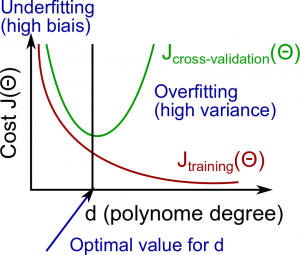
\includegraphics[scale=0.6]{W6_polydeg}
\caption{Polynomial degree}
\label{fig:W6_polydeg}
\end{figure}
\section{Regularization and Bias/Variance}
Instead of looking at the degree d contributing to bias/variance, now we will look at the regularization parameter $\lambda$.

\begin{itemize}
\item Large $\lambda$: High bias (underfitting)
\item Intermediate $\lambda$: just right
\item Small $\lambda$: High variance (overfitting)
\end{itemize}

A large lambda heavily penalizes all the $\Theta$ parameters, which greatly simplifies the line of our resulting function, so causes underfitting.

The relationship of $\lambda$ to the training set and the variance set is as follows:

\begin{itemize}
\item \textbf{Low $\lambda$}: $J_{train}(\Theta)$ is low and $J_{CV}(\Theta)$ is high (high variance/overfitting).
\item \textbf{Intermediate $\lambda$}: $J_{train}(\Theta)$ and $J_{CV}(\Theta)$ are somewhat low and $J_{train}(\Theta) \approx J_{CV}(\Theta)$
\item \textbf{Large $\lambda$}: both $J_{train}(\Theta)$ and $J_{CV}(\Theta)$ will be high (underfitting /high bias)
\end{itemize}

The figure \ref{fig:W6_polydeg2} illustrates the relationship between lambda and the hypothesis:

\begin{figure}[ht]
\center
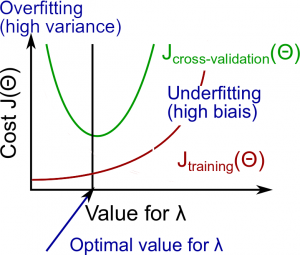
\includegraphics[scale=0.6]{W6_polydeg2}
\caption{relationship between lambda and the hypothesis}
\label{fig:W6_polydeg2}
\end{figure}

In order to choose the model and the regularization $\lambda$, we need:
\begin{enumerate}
\item Create a list of lambdas 

(i.e. $\lambda\in$\{0,0.01,0.02,0.04,0.08,
0.16,0.32,0.64,1.28,2.56,5.12,10.24\});
\item Create a set of models with different degrees or any other variants.
\item Iterate through the $\lambda$'s and for each $\lambda$ go through all the models to learn some $\Theta$.
\item Compute the cross validation error using the learned $\Theta$ (computed with $\lambda$) on the $J_{CV}(\Theta)$ without regularization or $\lambda = 0$.
\item Select the best combo that produces the lowest error on the cross validation set.
\item Using the best combo $\Theta$ and $\lambda$, apply it on $J_{test}(\Theta)$ to see if it has a good generalization of the problem.
\end{enumerate}
\section{Learning Curves}
Training 3 examples will easily have 0 errors because we can always find a quadratic curve that exactly touches 3 points.
\begin{itemize}
\item As the training set gets larger, the error for a quadratic function increases.
\item The error value will plateau out after a certain m, or training set size.
\end{itemize}
\subsection{With high bias}
\textbf{Low training set size}: causes $J_{train}(\Theta)$to be low and $J_{CV}(\Theta)$ to be high.

\textbf{Large training set size}: causes both $J_{train}(\Theta)$ and $J_{CV}(\Theta)$ to be high with $J_{train}(\Theta) \approx J_{CV}(\Theta)$

If a learning algorithm is suffering from \textbf{high bias}, getting more training data \textbf{will not (by itself) help much}.

For high variance, we have the following relationships in terms of the training set size:
\subsection{With high variance}
\textbf{Low training set size}: $J_{train}(\Theta)$ will be low and $J_{CV}(\Theta)$ will be high.

\textbf{Large training set size}: $J_{train}(\Theta)$ increases with training set size and $J_{CV}(\Theta)$ continues to decrease without leveling off. Also, $J_{train}(\Theta)<J_{CV}(\Theta)$ but the difference between them remains significant.

If a learning algorithm is suffering from \textbf{high variance}, getting more training data is \textbf{likely to help}.
\begin{figure}[ht]
     \centering
     \begin{subfigure}[b]{0.47\textwidth}
         \centering
         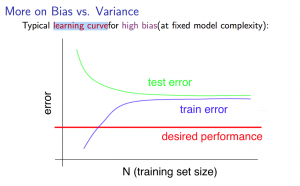
\includegraphics[width=\textwidth]{W6_LC1}
         \caption{More on Bias vs Variance}
         \label{fig:W6_LC1}
     \end{subfigure}
     \hfill
     \begin{subfigure}[b]{0.47\textwidth}
         \centering
         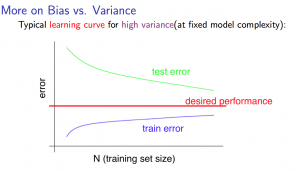
\includegraphics[width=\textwidth]{W6_LC2}
         \caption{More on Variance vs Bias}
         \label{fig:W6_LC2}
     \end{subfigure}
     \caption{Learning Curves}
     \label{fig:W6_LC}
\end{figure}

\section{Deciding What to Do Next Revisited}
Our decision process can be broken down as follows:
\begin{center}
\begin{tabular}{|c|c|}
\hline 
\textbf{Fixes High Bias} & \textbf{Fixes High Variance} \\ 
\hline 
Adding features & Getting more training examples \\ 
\hline 
Adding polynomial features & Trying smaller sets of features \\ 
\hline 
Decreasing $\lambda$ & Increasing $\lambda$ \\ 
\hline 
\end{tabular} 
\end{center}
\subsection{Diagnosing Neural Networks}
\begin{itemize}
\item A neural network with fewer parameters is prone to underfitting. It is also computationally cheaper.
\item A large neural network with more parameters is prone to overfitting. It is also computationally expensive. In this case you can use regularization (increase $\lambda$) to address the overfitting.
\end{itemize}
Using a single hidden layer is a good starting default. You can train your neural network on a number of hidden layers using your cross validation set.

\subsection{Model Selection}
Choosing M the order of polynomials.

How can we tell which parameters $\Theta$ to leave in the model (known as ``model selection")?

There are several ways to solve this problem:

\begin{itemize}
\item Get more data (\textbf{very difficult}).
\item Choose the model which best fits the data without overfitting (\textbf{very difficult}).
\item Reduce the opportunity for overfitting through regularization.
\end{itemize}

\subsubsection{Bias: approximation error (Difference between expected value and optimal value)}
\begin{itemize}
\item High Bias = UnderFitting (BU)
\item $J_{train}(\Theta)$ both will be high and $J_{train}(\Theta)\approx J_{CV}(\Theta)$
\end{itemize}
\subsubsection{Variance: estimation error due to finite data}
\begin{itemize}
\item High Variance = OverFitting (VO)
\item $J_{train}(\Theta)$ is low and $J_{CV}(\Theta) \gg J_{train}(\Theta)$
\end{itemize}
\subsubsection{Intuition for the bias-variance trade-off:}
\begin{itemize}
\item Complex model $=>$ sensitive to data $=>$ much affected by changes in X $=>$ high variance, low bias.
\item Simple model $=>$ more rigid $=>$ does not change as much with changes in X $=>$ low variance, high bias.
\end{itemize}

One of the most important goals in learning: finding a model that is just right in the bias-variance trade-off.

\subsubsection{Regularization effects}
\begin{itemize}
\item Small values of $\lambda$ allow model to become finely tuned to noise leading to large variance $=>$ overfitting.
\item Large values of $\lambda$ pull weight parameters to zero leading to large bias $=>$ underfitting.
\end{itemize}

\subsubsection{Model Complexity Effects}
\begin{itemize}
\item Lower-order polynomials (low model complexity) have high bias and low variance. In this case, the model fits poorly consistently.
\item Higher-order polynomials (high model complexity) fit the training data extremely well and the test data extremely poorly. These have low bias on the training data, but very high variance.
\item In reality, we would want to choose a model somewhere in between, that can generalize well but also fits the data reasonably well.
\end{itemize}

\subsubsection{A typical rule of thumb when running diagnostics is:}
\begin{itemize}
\item More training examples fixes high variance but not high bias.
\item Fewer features fixes high variance but not high bias.
\item Additional features fixes high bias but not high variance.
\item The addition of polynomial and interaction features fixes high bias but not high variance.
\item When using gradient descent, decreasing lambda can fix high bias and increasing lambda can fix high variance (lambda is the regularization parameter).
\item When using neural networks, small neural networks are more prone to under-fitting and big neural networks are prone to over-fitting. Cross-validation of network size is a way to choose alternatives.
\end{itemize}

\section{ML: Machine Learning System Design}
\subsection{Prioritizing What to work On}
Different ways we can approach a machine learning problem:
\begin{itemize}
\item Collect lots of data (for example "honeypot" project but doesn't always work)
\item Develop sophisticated features (for example: using email header data in spam emails)
\item Develop algorithms to process your input in different ways (recognizing misspellings in spam).
\end{itemize}

It is difficult to tell which of the options will be helpful.
\subsection{Error Analysis}
The recommended approach to solving machine learning problems is:
\begin{itemize}
\item Start with a simple algorithm, implement it quickly, and test it early.
\item Plot learning curves to decide if more data, more features, etc. will help
\item Error analysis: manually examine the errors on examples in the cross validation set and try to spot a trend.
\end{itemize}
It's important to get error results as a single, numerical value. Otherwise it is difficult to assess your algorithm's performance.

You may need to process your input before it is useful. For example, if your input is a set of words, you may want to treat the same word with different forms (fail/failing/failed) as one word, so must use "stemming software" to recognize them all as one.
\subsection{Error Metrics for Skewed Classes}
It is sometimes difficult to tell whether a reduction in error is actually an improvement of the algorithm.
\begin{itemize}
\item For example: In predicting a cancer diagnoses where 0.5\% of the examples have cancer, we find our learning algorithm has a 1\% error. However, if we were to simply classify every single example as a 0, then our error would reduce to 0.5\% even though we did not improve the algorithm.
\end{itemize}

This usually happens with skewed classes; that is, when our class is very rare in the entire data set.

Or to say it another way, when we have lot more examples from one class than from the other class.

For this we can use Precision/Recall.
\begin{itemize}
\item Predicted: 1, Actual: 1 --- True positive
\item Predicted: 0, Actual: 0 --- True negative
\item Predicted: 0, Actual, 1 --- False negative
\item Predicted: 1, Actual: 0 --- False positive
\end{itemize}

\textbf{Precision}: of all patients we predicted where y=1, what fraction actually has cancer?
\begin{equation}
\dfrac{\text{True Positives}}{\text{Total number of predicted positives}}
= \dfrac{\text{True Positives}}{\text{True Positives}+\text{False positives}}
\end{equation}

\textbf{Recall}: Of all the patients that actually have cancer, what fraction did we correctly detect as having cancer?

\begin{equation}
\dfrac{\text{True Positives}}{\text{Total number of actual positives}}= \dfrac{\text{True Positives}}{\text{True Positives}+\text{False negatives}} 
\end{equation}
These two metrics give us a better sense of how our classifier is doing. We want both precision and recall to be high.

In the example at the beginning of the section, if we classify all patients as 0, then our recall will be $\dfrac{0}{0 + f} = 0 $, so despite having a lower error percentage, we can quickly see it has worse recall.

\[
 \text{Accuracy } = \frac {true positive + true negative} {total population} 
\]
\textbf{Note} 1: if an algorithm predicts only negatives like it does in one of exercises, the precision is not defined, it is impossible to divide by 0. F1 score will not be defined too.

\section{Trading off Precision and Recall}
We might want a \textbf{confident} prediction of two classes using logistic regression. One way is to increase our threshold:
\begin{itemize}
\item Predict 1 if: $h_\theta(x) \geq 0.7$
\item Predict 0 if: $h_\theta(x) < 0.7$
\end{itemize}
This way, we only predict cancer if the patient has a 70% chance.

Doing this, we will have higher precision but lower recall (refer to the definitions in the previous section).

In the opposite example, we can lower our threshold:
\begin{itemize}
\item Predict 1 if: $h_\theta(x) \geq 0.3$
\item Predict 0 if: $h_\theta(x) < 0.3$
\end{itemize}

That way, we get a very \textbf{safe} prediction. This will cause \textbf{higher recall} but \textbf{lower precision}.

The greater the threshold, the greater the precision and the lower the recall.

The lower the threshold, the greater the recall and the lower the precision.

In order to turn these two metrics into one single number, we can take the \textbf{F value}.

One way is to take the average:
$$\dfrac{P+R}{2} $$

This does not work well. If we predict all y=0 then that will bring the average up despite having 0 recall. If we predict all examples as y=1, then the very high recall will bring up the average despite having 0 precision.

A better way is to compute the \textbf{F Score} (or F1 score):

$$\text{F Score} = 2\dfrac{PR}{P + R}$$
In order for the F Score to be large, both precision and recall must be large.

We want to train precision and recall on the \textbf{cross validation set} so as not to bias our test set.
\section{Data for Machine Learning}
How much data should we train on?

In certain cases, an ``inferior algorithm," if given enough data, can outperform a superior algorithm with less data.

We must choose our features to have enough information. A useful test is: Given input x, would a human expert be able to confidently predict y?

\textbf{Rationale for large data}: if we have a \textbf{low bias} algorithm (many features or hidden units making a very complex function), then the larger the training set we use, the less we will have overfitting (and the more accurate the algorithm will be on the test set). 
\section{Quiz Instructions}
When the quiz instructions tell you to enter a value to ``two decimal digits", what it really means is ``two significant digits". So, just for example, the value 0.0123 should be entered as ``0.012", not ``0.01".

\subsection*{References}
\begin{itemize}
\item \href{https://class.coursera.org/ml/lecture/index}{Coursera}
\item \href{http://www.cedar.buffalo.edu/~srihari/CSE555/Chap9.Part2.pdf}{Bias/Variance University at Buffalo}
\item \href{https://blog.stephenpurpura.com/post/13052575854/managing-bias-variance-tradeoff-in-machine}{Managing Bias - Variance (Abductive Intelligence)}
\end{itemize}
\chapter{Week 7}
\section{Optimization Objective}
The \textbf{Support Vector Machine} (SVM) is yet another type of supervised machine learning algorithm. It is sometimes cleaner and more powerful.

Recall that in logistic regression, we use the following rules:

\begin{itemize}
\item y=1, then $h_\theta(x) \approx 1$ and $\Theta^Tx \gg 0$
\item y=0, then $h_\theta(x) \approx 0$ and $\Theta^Tx \ll 0$
\end{itemize}
Recall the cost function for (unregularized) logistic regression:
 
\begin{align*}
J(\theta) 
& = \frac{1}{m}\sum_{i=1}^m -y^{(i)} \log(h_\theta(x^{(i)})) - (1 - y^{(i)})\log(1 - h_\theta(x^{(i)}))\\ 
& = \frac{1}{m}\sum_{i=1}^m -y^{(i)} \log\Big(\dfrac{1}{1 + e^{-\theta^Tx^{(i)}}}\Big) - (1 - y^{(i)})\log\Big(1 - \dfrac{1}{1 + e^{-\theta^Tx^{(i)}}}\Big)
\end{align*}
To make a support vector machine, we will modify the first term of the cost function $$-\log(h_{\theta}(x)) = -\log\Big(\dfrac{1}{1 + e^{-\theta^Tx}}\Big)$$ (figure \ref{fig:W7_1}) so that when $\Theta^Tx$(from now on, we shall refer to this as z) \textbf{is greater than 1}, it outputs 0. Furthermore, for values of z less than 1, we shall use a straight decreasing line instead of the sigmoid curve. In the literature, this is called a \href{https://en.wikipedia.org/wiki/Hinge_loss}{hinge loss} function.

Similarly, we modify the second term of the cost function $$-\log(1 - h_{\theta(x)}) = -\log\Big(1 - \dfrac{1}{1 + e^{-\theta^Tx}}\Big)$$ (figure \ref{fig:W7_2}). so that when z is less than -1, it outputs 0. We also modify it so that for values of z greater than -1, we use a straight increasing line instead of the sigmoid curve.

\begin{figure}[ht]
     \centering
     \begin{subfigure}[b]{0.35\textwidth}
         \centering
         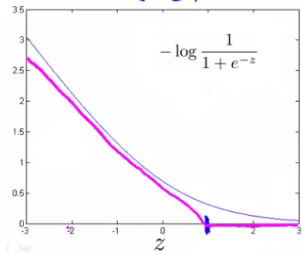
\includegraphics[width=\textwidth]{W7_1}
         \caption{}
         \label{fig:W7_1}
     \end{subfigure}
     \begin{subfigure}[b]{0.35\textwidth}
         \centering
         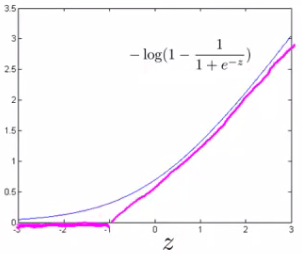
\includegraphics[width=\textwidth]{W7_2}
         \caption{}
         \label{fig:W7_2}
     \end{subfigure}
        \caption{}
        \label{fig:}
\end{figure}

We shall denote these as $\text{cost}_1(z)$ and $\text{cost}_0(z)$ (respectively, note that $\text{cost}_1(z)$ is the cost for classifying when y=1, and $\text{cost}_0(z)$ is the cost for classifying when y=0), and we may define them as follows (where k is an arbitrary constant defining the magnitude of the slope of the line):

$$z = \theta^Tx$$
$$\text{cost}_0(z) = \max(0, k(1+z))$$
$$\text{cost}_1(z) = \max(0, k(1-z))$$
Recall the full cost function from (regularized) logistic regression:
\begin{equation}
J(\theta) = \frac{1}{m} \sum_{i=1}^m y^{(i)}(-\log(h_\theta(x^{(i)}))) + (1 - y^{(i)})(-\log(1 - h_\theta(x^{(i)}))) + \dfrac{\lambda}{2m}\sum_{j=1}^n \Theta^2_jJ
\end{equation}
Note that the negative sign has been distributed into the sum in the above equation.

We may transform this into the cost function for support vector machines by substituting $\text{cost}_0(z)$ and $\text{cost}_1(z)$:

\begin{equation}
J(\theta) = \frac{1}{m} \sum_{i=1}^m y^{(i)} \ \text{cost}_1(\theta^Tx^{(i)}) + (1 - y^{(i)}) \ \text{cost}_0(\theta^Tx^{(i)}) + \dfrac{\lambda}{2m}\sum_{j=1}^n \Theta^2_j
\end{equation}

We can optimize this a bit by multiplying this by m (thus removing the m factor in the denominators). Note that this does not affect our optimization, since we're simply multiplying our cost function by a positive constant (for example, minimizing $(u-5)^2 + 1$ gives us 5; multiplying it by 10 to make it $10(u-5)^2 + 10$ still gives us 5 when minimized).
\begin{equation}
J(\theta) = \sum_{i=1}^m y^{(i)} \ \text{cost}_1(\theta^Tx^{(i)}) + (1 - y^{(i)}) \ \text{cost}_0(\theta^Tx^{(i)}) + \dfrac{\lambda}{2}\sum_{j=1}^n \Theta^2_j
\end{equation}

This is equivalent to multiplying the equation by $C = \dfrac{1}{\lambda}$, and thus results in the same values when optimized. Now, when we wish to regularize more (that is, reduce overfitting), we decrease C, and when we wish to regularize less (that is, reduce underfitting), we increase C.

Finally, note that the hypothesis of the Support Vector Machine is not interpreted as the probability of y being 1 or 0 (as it is for the hypothesis of logistic regression). Instead, it outputs either 1 or 0. (In technical terms, it is a discriminant function.)
\begin{equation}
h_\theta(x) = \begin{cases}1 & \text{if}\quad \Theta^Tx\ge0 \\0 &\text{if}\quad \text{otherwise}\end{cases}
\end{equation}

\section{Large Margin Intuition}
A useful way to think about Support Vector Machines is to think of them as Large Margin Classifiers.
\begin{itemize}
\item If y=1, we want $\Theta^Tx \geq 1$ (not just $\ge$ 0)
\item If y=0, we want $\Theta^Tx \leq 1$ (not just $<$ 0)
\end{itemize}

Now when we set our constant C to a very large value (e.g. 100,000), our optimizing function will constrain $\Theta$ such that the equation A (the summation of the cost of each example) equals 0. We impose the following constraints on $\Theta$:

$\Theta^Tx \geq 1$ if y=1 and $\Theta^Tx \leq -1$ if y=0.

If C is very large, we must choose $\Theta$ parameters such that:
\[\sum_{i=1}^m y^{(i)}\text{cost}_1(\Theta^Tx) + (1 - y^{(i)})\text{cost}_0(\Theta^Tx) = 0\]
This reduces our cost function to:
\begin{align*}
J(\theta) = C \cdot 0 + \dfrac{1}{2}\sum_{j=1}^n \Theta^2_j \newline
= \dfrac{1}{2}\sum_{j=1}^n \Theta^2_j
\end{align*}
Recall the decision boundary from logistic regression (the line separating the positive and negative examples). In SVMs, the decision boundary has the special property that it is \textbf{as far away as possible} from both the positive and the negative examples.

The distance of the decision boundary to the nearest example is called the \textbf{margin}. Since SVMs maximize this margin, it is often called a Large Margin Classifier.

The SVM will separate the negative and positive examples by a \textbf{large margin}.

This large margin is only achieved when C is very large.

Data is \textbf{linearly separable} when a \textbf{straight line} can separate the positive and negative examples.

If we have \textbf{outlier} examples that we don't want to affect the decision boundary, then we can \textbf{reduce} C.

Increasing and decreasing C is similar to respectively decreasing and increasing $\lambda$, and can simplify our decision boundary.
\section{Mathematics Behind Large Margin Classification}
\subsection{Vector Inner Product}
Say we have two vectors, u and v:

\begin{align*}
u = 
\begin{bmatrix}
u_1 \\ u_2
\end{bmatrix}
v = 
\begin{bmatrix}
v_1 \\ v_2
\end{bmatrix}
\end{align*}

The \textbf{length of vector v} is denoted $\parallel v\parallel$, and it describes the line on a graph from origin (0,0) to $(v_1,v_2)$

The length of vector v can be calculated with $\sqrt{v_1^2 + v_2^2}$ by the Pythagorean theorem.

The \textbf{projection} of vector v onto vector u is found by taking a right angle from u to the end of v, creating a right triangle.

\begin{itemize}
\item p = length of projection of v onto the vector u.
\item $u^Tv = p \cdot \parallel v \parallel$
\end{itemize}

Note that  $u^Tv = ||u|| \cdot ||v|| \cos \theta$ where $\theta$ is the angle between u and v. Also, $p = ||v|| \cos \theta$. If you substitute $p$ for $||v|| \cos \theta$ you get $u^Tv= p \cdot ||u||$.

So the product $u^Tv$ is equal to the length of the projection times the length of vector u.

In our example, since u and v are vectors of the same length, $u^Tv = v^Tu$.

$u^Tv = v^Tu = p \cdot ||u|| = u_1v_1 + u_2v_2$

If the \textbf{angle} between the lines for $v$ and $u$ is \textbf{greater than 90 degrees}, then the projection $p$ will be negative.
\begin{align*}
&\min_\Theta \dfrac{1}{2}\sum_{j=1}^n \Theta_j^2 \\
&= \dfrac{1}{2}(\Theta_1^2 + \Theta_2^2 + \dots + \Theta_n^2) \\
&= \dfrac{1}{2}(\sqrt{\Theta_1^2 + \Theta_2^2 + \dots + \Theta_n^2})^2 \\
&= \dfrac{1}{2}||\Theta ||^2 \\
\end{align*}

We can use the same rules to rewrite $\Theta^Tx^{(i)}$
\[
\Theta^Tx^{(i)} = p^{(i)} \cdot ||\Theta || = \Theta_1x_1^{(i)} + \Theta_2x_2^{(i)} + \dots + \Theta_n x_n^{(i)}
\]

So we now have a new optimization objective by substituting $p^{(i)} \cdot ||\Theta ||$ in for $\Theta^Tx^{(i)}$
\begin{itemize}
\item If y=1, we want $p^{(i)} \cdot ||\Theta || \geq 1$
\item If y=0, we want $p^{(i)} \cdot ||\Theta || \leq -1$
\end{itemize}

The reason this causes a ``large margin" is because: the vector for $\Theta$ is perpendicular to the decision boundary. In order for our optimization objective (above) to hold true, we need the absolute value of our projections $p^{(i)}$ to be as large as possible.

If $\Theta_0 =0$, then all our decision boundaries will intersect (0,0). If $\Theta_0 \neq 0$, the support vector machine will still find a large margin for the decision boundary.

\section{Kernels I}
Kernels allow us to make complex, non-linear classifiers using Support Vector Machines.

Given x, compute new feature depending on proximity to landmarks $l^{(1)},\ l^{(2)},\ l^{(3)}$

To do this, we find the ``similarity" of $x$ and some landmark $l^{(i)}$s:
\[
f_i = similarity(x, l^{(i)}) = \exp(-\dfrac{\sum^n_{j=1}(x_j-l_j^{(i)})^2}{2\sigma^2})
\]

There are a couple properties of the similarity function:

If $x \approx l^{(i)}$), then $f_i = \exp(-\dfrac{\approx 0^2}{2\sigma^2}) \approx 1$

If x is far from $l^{(i)}$, then $f_i = \exp(-\dfrac{(large\ number)^2}{2\sigma^2}) \approx 0$

In other words, if x and the landmark are close, then the similarity will be close to 1, and if x and the landmark are far away from each other, the similarity will be close to 0.

Each landmark gives us the features in our hypothesis:


\begin{align*}l^{(1)} \rightarrow f_1 \newline l^{(2)} \rightarrow f_2 \\
 l^{(3)} \rightarrow f_3 \\
\dots \\
 h_\Theta(x) = \Theta_1f_1 + \Theta_2f_2 + \Theta_3f_3 + \dots
\end{align*}

$\sigma^2$is a parameter of the Gaussian Kernel, and it can be modified to increase or decrease the \textbf{drop-off} of our feature $f_i$. Combined with looking at the values inside $\Theta$, we can choose these landmarks to get the general shape of the decision boundary.

\section{Kernels II}
One way to get the landmarks is to put them in the \textbf{exact same} locations as all the training examples. This gives us m landmarks, with one landmark per training example.

Given example x:

$f_1 = similarity(x,l^{(1)})$, $f_2 = similarity(x,l^{(2)})$, $f_3 = similarity(x,l^{(3)})$, and so on.

This gives us a ``feature vector", $f_{(i)}$ of all our features for example $x_{(i)}$. We may also set $f_0 = 1$ to correspond with $\Theta_0$. Thus given training example $x_{(i)}$:

$$x^{(i)} \rightarrow f^{(i)}_1=similarity(x^{(i)},l^{(1)})f^{(i)}_2$$
$$=similarity(x^{(i)},l^{(2)})\cdots f^{(i)}_m$$
$$=similarity(x^{(i)},l^{(m)})$$

Now to get the parameters $\Theta$ we can use the \textbf{SVM} minimization algorithm but with $f^{(i)}$ substituted in for $x^{(i)}$:
$$
\min_{\Theta} C \sum_{i=1}^m y^{(i)}\text{cost}_1(\Theta^Tf^{(i)}) + (1 - y^{(i)})\text{cost}_0(\theta^Tf^{(i)}) + \dfrac{1}{2}\sum_{j=1}^n \Theta^2_j
$$
Using kernels to generate f(i) is not exclusive to SVMs and may also be applied to logistic regression. However, because of computational optimizations on SVMs, kernels combined with SVMs is much faster than with other algorithms, so kernels are almost always found combined only with SVMs.
\subsection{Choosing SVM parameters}
Choosing C (recall that $C = \dfrac{1}{\lambda}$)
\begin{itemize}
\item If C is large, then we get higher variance/lower bias
\item If C is small, then we get lower variance/higher bias
\end{itemize}

The other parameter we must choose is $\sigma^2$ from the Gaussian Kernel function:
\begin{itemize}
\item With a large $\sigma^2$, the features fi vary more smoothly, causing higher bias and lower variance.
\item With a small $\sigma^2$, the features fi vary less smoothly, causing lower bias and higher variance.
\end{itemize}

\subsection{Using An SVM}

There are lots of good SVM libraries already written. A. Ng often uses `\textbf{liblinear}' and `\textbf{libsvm}'. In practical application, you should use one of these libraries rather than rewrite the functions.

In practical application, the choices you do need to make are:
\begin{itemize}
	\item Choice of parameter C
	\item Choice of kernel (similarity function)
	\item No kernel (``linear" kernel) -- gives standard linear classifier
	\item Choose when n is large and when m is small
	\item Gaussian Kernel (above) -- need to choose $\sigma^2$ 
	\item Choose when n is small and m is large
\end{itemize}

The library may ask you to provide the kernel function.

\textbf{Note}: do perform feature scaling before using the Gaussian Kernel.

\textbf{Note}: not all similarity functions are valid kernels. They must satisfy ``Mercer's Theorem" which guarantees that the SVM package's optimizations run correctly and do not diverge.

You want to train C and the parameters for the kernel function using the training and cross-validation datasets.

\subsection{Multi-class Classification}
Many SVM libraries have multi-class classification built-in.

You can use the one-vs-all method just like we did for logistic regression, where $y \in {1,2,3,\dots,K}$ with $\Theta^{(1)}, \Theta^{(2)}, \dots,\Theta{(K)}$. We pick class $i$ with the largest ($\Theta^{(i)})^Tx$.

\subsection{Logistic Regression vs. SVMs}
If n is large (relative to m), then use logistic regression, or SVM without a kernel (the ``linear kernel")

If n is small and m is intermediate, then use SVM with a Gaussian Kernel

If n is small and m is large, then manually create/add more features, then use logistic regression or SVM without a kernel.

In the first case, we don't have enough examples to need a complicated polynomial hypothesis. In the second example, we have enough examples that we may need a complex non-linear hypothesis. In the last case, we want to increase our features so that logistic regression becomes applicable.

\textbf{Note}: a neural network is likely to work well for any of these situations, but may be slower to train.

\subsubsection{Additional references}
\begin{itemize}
\item \href{http://web.mit.edu/6.034/wwwbob/svm-notes-long-08.pdf}{An Idiot's Guide to Support Vector Machines}
\end{itemize}
\chapter{Week 8}
\section{Machine Learning: Clustering}
\section{Unsupervised Learning: Introduction}
Unsupervised learning is contrasted from supervised learning because it uses an unlabeled training set rather than a labeled one.

In other words, we don't have the vector y of expected results, we only have a dataset of features where we can find structure.

Clustering is good for:
\begin{itemize}
	\item Market segmentation
	\item Social network analysis
	\item Organizing computer clusters
	\item Astronomical data analysis
\end{itemize}

\section{K-Means Algorithm}
The K-Means Algorithm is the most popular and widely used algorithm for automatically grouping data into coherent subsets.
\begin{enumerate}
	\item Randomly initialize two points in the dataset called the cluster centroids.
	\item Cluster assignment: assign all examples into one of two groups based on which cluster centroid the example is closest to.
	\item Move centroid: compute the averages for all the points inside each of the two cluster centroid groups, then move the cluster centroid points to those averages.
	\item Re-run (2) and (3) until we have found our clusters.
\end{enumerate}
Our main variables are:
\begin{itemize}
	\item K (number of clusters)
	\item Training set $ x^{(1)}, x^{(2)}, \dots, x^{(m)} $
	\item Where $x^{(i)} \in \mathbb{R}^n$
\end{itemize}

Note that we will not use the x0=1 convention.

\subsection{The algorithm:}
\begin{verbatim}
Randomly initialize K cluster centroids mu(1), mu(2), ..., mu(K)
Repeat:
   for i = 1 to m:
      c(i):= index (from 1 to K) of cluster centroid closest to x(i)
   for k = 1 to K:
      mu(k):= average (mean) of points assigned to cluster k
\end{verbatim}
The \textbf{first for-loop} is the `Cluster Assignment' step. We make a vector c where c(i) represents the centroid assigned to example x(i).

We can write the operation of the Cluster Assignment step more mathematically as follows:

\begin{equation}
c^{(i)} = argmin_k\ ||x^{(i)} - \mu_k||^2
\end{equation}

That is, each $c^{(i)}$ contains the index of the centroid that has minimal distance to $x^{(i)}$.

By convention, we square the right-hand-side, which makes the function we are trying to minimize more sharply increasing. It is mostly just a convention. But a convention that helps reduce the computation load because the Euclidean distance requires a square root but it is canceled.

Without the square:
\begin{equation}
||x^{(i)} - \mu_k|| = ||\quad\sqrt{(x_1^i - \mu_{1(k)})^2 + (x_2^i - \mu_{2(k)})^2 + (x_3^i - \mu_{3(k)})^2 + ...}\quad||
\end{equation}

With the square:
\begin{equation}
||x^{(i)} - \mu_k||^2 = ||\quad(x_1^i - \mu_{1(k)})^2 + (x_2^i - \mu_{2(k)})^2 + (x_3^i - \mu_{3(k)})^2 + ...\quad||
\end{equation}
...so the square convention serves two purposes, minimize more sharply and less computation.

The \textbf{second for-loop} is the `Move Centroid' step where we move each centroid to the average of its group.

More formally, the equation for this loop is as follows:
\begin{equation}
\mu_k = \dfrac{1}{n}[x^{(k_1)} + x^{(k_2)} + \dots + x^{(k_n)}] \in \mathbb{R}^n
\end{equation}
If you have a cluster centroid with \textbf{0 points} assigned to it, you can randomly \textbf{re-initialize} that centroid to a new point. You can also simply \textbf{eliminate} that cluster group.

After a number of iterations the algorithm will \textbf{converge}, where new iterations do not affect the clusters.

Note on non-separated clusters: some datasets have no real inner separation or natural structure. K-means can still evenly segment your data into K subsets, so can still be useful in this case.
\section{Optimization Objective}
Recall some of the parameters we used in our algorithm:
\begin{itemize}
	\item $c^{(i)}$ = index of cluster (1,2,...,K) to which example x(i) is currently assigned
	\item $\mu_k$ = cluster centroid $k(\mu k\in \mathbb{R}n)$
	\item $\mu_{c^{(i)}}$ = cluster centroid of cluster to which example x(i) has been assigned
\end{itemize}

Using these variables we can define our cost function:
\begin{equation}
J(c^{(i)},\dots,c^{(m)},\mu_1,\dots,\mu_K) = \dfrac{1}{m}\sum_{i=1}^m ||x^{(i)} - \mu_{c^{(i)}}||^2
\end{equation}
Our optimization objective is to minimize all our parameters using the above cost function:

$$min_{c,\mu}\ J(c,\mu)$$
That is, we are finding all the values in sets c, representing all our clusters, and $\mu$, representing all our centroids, that will minimize the \textbf{average of the distances} of every training example to its corresponding cluster centroid.

The above cost function is often called the \textbf{distortion} of the training examples.

In the \textbf{cluster assignment step}, our goal is to:
\begin{itemize}
	\item Minimize J(…) with $c^{(1)},\dots,c^{(m)}$ (holding $\mu_1,\dots,\mu_K$ fixed)
\end{itemize}

In the move centroid step, our goal is to:
\begin{itemize}
	\item Minimize J(…) with $\mu_1,\dots,\mu_K$
\end{itemize}

With k-means, it \textbf{is not possible for the cost function to sometimes increase}. It should always descend.

\section{Random Initialization}

\chapter{ML - Anomaly Detection}

\section{Problem Motivation}
Just like in other learning problems, we are given a dataset ${x^{(1)}, x^{(2)},\dots,x^{(m)}}$.

We are then given a new example, $x_{test}$, and we want to know whether this new example is abnormal/anomalous.

We define a ``model" p(x) that tells us the probability the example is not anomalous. We also use a threshold $\epsilon$ (epsilon) as a dividing line so we can say which examples are anomalous and which are not.

A very common application of anomaly detection is detecting fraud:

\begin{itemize}
\item $x^{(i)} = $features of user i's activities.
\item Model p(x) from the data.
\item Identify unusual users by checking $ p(x) < \epsilon$
\end{itemize}

If our anomaly detector is flagging \textbf{too many} anomalous examples, then we need to \textbf{decrease} our threshold $\epsilon$

\section{Gaussian Distribution}
The Gaussian Distribution is a familiar bell-shaped curve that can be described by a function 
$$\mathcal{N}(\mu,\sigma^2)$$

Let $x\in \mathbb{R}$. If the probability distribution of x is Gaussian with mean $\mu$, variance $\sigma^2$, then:

\begin{equation}
x \sim \mathcal{N}(\mu, \sigma^2)
\end{equation}

The little $\sim$ or `tilde' can be read as ``distributed as".


The Gaussian Distribution is parameterized by a mean and a variance.

$\mu$, describes the center of the curve, called the mean. The width of the curve is described by $\sigma$, called the standard deviation.

The full function is as follows:

\begin{equation}
p(x;\mu,\sigma^2) = \dfrac{1}{\sigma\sqrt{(2\pi)}}e^{-\dfrac{1}{2}(\dfrac{x - \mu}{\sigma})^2}
\end{equation}

We can estimate the parameter $\mu$ from a given dataset by simply taking the average of all the examples:
\begin{equation}
\mu = \dfrac{1}{m}\displaystyle \sum_{i=1}^m x^{(i)}
\end{equation}

We can estimate the other parameter, $\sigma^2$, with our familiar squared error formula:
\begin{equation}
\sigma^2 = \dfrac{1}{m}\displaystyle \sum_{i=1}^m(x^{(i)} - \mu)^2
\end{equation}

\section{Algorithm}
Given a training set of examples, $\lbrace x^{(1)},\dots,x^{(m)}\rbrace $ where each example is a vector, $x \in \mathbb{R}$.
\begin{equation}
p(x) = p(x_1;\mu_1,\sigma_1^2)p(x_2;\mu_2,\sigma^2_2)\cdots p(x_n;\mu_n,\sigma^2_n)
\end{equation}

\subsection{The algorithm}
Choose features $x_i$ that you think might be indicative of anomalous examples.

Fit parameters $\mu_1,\dots,\mu_n,\sigma_1^2,\dots,\sigma_n^2$

Calculate $\mu_j = \dfrac{1}{m}\displaystyle \sum_{i=1}^m x_j^{(i)}$

Calculate $\sigma^2_j = \dfrac{1}{m}\displaystyle \sum_{i=1}^m(x_j^{(i)} - \mu_j)^2$

Given a new example x, compute p(x):
\begin{equation}
p(x) = \displaystyle \prod^n_{j=1} p(x_j;\mu_j,\sigma_j^2) = \prod\limits^n_{j=1} \dfrac{1}{\sqrt{2\pi}\sigma_j}exp(-\dfrac{(x_j - \mu_j)^2}{2\sigma^2_j})
\end{equation}

{\bf Anomaly} if $p(x) < \epsilon$

A vectorized version of the calculation for $\mu$ is $\mu = \dfrac{1}{m}\displaystyle \sum_{i=1}^m x^{(i)}$

You can vectorize $\sigma^2$ similarly.

\section{Developing and Evaluating an Anomaly Detection System}
To evaluate our learning algorithm, we take some labeled data, categorized into anomalous and non-anomalous examples ( y = 0 if normal, y = 1 if anomalous).

Among that data, take a large proportion of good, non-anomalous data for the training set on which to train p(x).

Then, take a smaller proportion of mixed anomalous and non-anomalous examples (you will usually have many more non-anomalous examples) for your cross-validation and test sets.

For example, we may have a set where 0.2\% of the data is anomalous. We take 60\% of those examples, all of which are good (y=0) for the training set. We then take 20\% of the examples for the cross-validation set (with 0.1\% of the anomalous examples) and another 20\% from the test set (with another 0.1\% of the anomalous).

In other words, we split the data 60/20/20 training/CV/test and then split the anomalous examples 50/50 between the CV and test sets.

\subsection{Algorithm evaluation}

Fit model $p(x)$ on training set $\lbrace x^{(1)},\dots,x^{(m)} \rbrace$.

On a cross validation/test example x, predict:

If $p(x) < \epsilon$ (\textbf{anomaly}), then y=1

If $p(x) \geq \epsilon $(\textbf{normal}), then y=0

Possible evaluation metrics (see ``Machine Learning System Design" section):

\begin{itemize}
\item True positive, false positive, false negative, true negative.
\item Precision/recall
\item $F_1$ score 
\end{itemize}

Note that we use the cross-validation set to choose parameter $\epsilon$

\section{Anomaly Detection vs. Supervised Learning}
When do we use anomaly detection and when do we use supervised learning?

\subsection{Use anomaly detection when...}
\begin{itemize}
\item We have a very small number of positive examples (y=1 ... 0-20 examples is common) and a large number of negative (y=0) examples.
\item We have many different ``types" of anomalies and it is hard for any algorithm to learn from positive examples what the anomalies look like; future anomalies may look nothing like any of the anomalous examples we've seen so far.
\end{itemize}

\subsection{Use supervised learning when...}
\begin{itemize}
\item We have a large number of both positive and negative examples. In other words, the training set is more evenly divided into classes.
\item We have enough positive examples for the algorithm to get a sense of what new positives examples look like. The future positive examples are likely similar to the ones in the training set.
\end{itemize}

\section{Choosing What Features to Use}
he features will greatly affect how well your anomaly detection algorithm works.

We can check that our features are \textbf{gaussian} by plotting a histogram of our data and checking for the bell-shaped curve.

Some \textbf{transforms} we can try on an example feature x that does not have the bell-shaped curve are:

\begin{itemize}
\item $\log(x)$
\item $\log(x+1)$
\item $\log(x+c)$ for some constant
\item $\sqrt{x}$
\item $x^{1/3}$
\end{itemize}

We can play with each of these to try and achieve the gaussian shape in our data.

There is an \textbf{error analysis procedure} for anomaly detection that is very similar to the one in supervised learning.

Our goal is for p(x) to be large for normal examples and small for anomalous examples.

One common problem is when p(x) is similar for both types of examples. In this case, you need to examine the anomalous examples that are giving high probability in detail and try to figure out new features that will better distinguish the data.

In general, choose features that might take on unusually large or small values in the event of an anomaly.

\section{Multivariate Gaussian Distribution (Optional)}
The multivariate gaussian distribution is an extension of anomaly detection and may (or may not) catch more anomalies.

Instead of modeling $p(x_1),p(x_2),\dots$ separately, we will model p(x) all in one go. Our parameters will be: $\mu \in \mathbb{R}^n$, and $\Sigma \in \mathbb{R}^{n \times n}$

\begin{equation}
p(x;\mu,\Sigma) = \dfrac{1}{(2\pi)^{n/2} |\Sigma|^{1/2}} exp(-1/2(x-\mu)^T\Sigma^{-1}(x-\mu))
\end{equation}

The important effect is that we can model oblong gaussian contours, allowing us to better fit data that might not fit into the normal circular contours.

Varying $\Sigma$ changes the shape, width, and orientation of the contours. Changing $\mu$ will move the center of the distribution.

Check also:
\begin{itemize}
\item[[1]] \href{http://cs229.stanford.edu/section/gaussians.pdf}{The Multivariate Gaussian Distribution}, Chuong B. Do, October 10, 2008.
\end{itemize}

\section{Anomaly Detection using the Multivariate Gaussian Distribution (Optional)}
When doing anomaly detection with multivariate gaussian distribution, we compute $\mu$ and $\Sigma$ normally. We then compute $p(x)$ using the new formula in the previous section and flag an anomaly if $p(x) < \epsilon$.

The original model for $p(x)$ corresponds to a multivariate Gaussian where the contours of $p(x;\mu,\Sigma)$ are axis-aligned.

The multivariate Gaussian model can automatically capture correlations between different features of $x$.

However, the original model maintains some advantages: it is computationally cheaper (no matrix to invert, which is costly for large number of features) and it performs well even with small training set size (in multivariate Gaussian model, it should be greater than the number of features for $\Sigma$ to be invertible).

\section{ML: Recommender Systems}
\subsection{Problem Formulation}
Recommendation is currently a very popular application of machine learning.

Say we are trying to recommend movies to customers. We can use the following definitions:
\begin{itemize}
\item $n_u =$ number of users.
\item $n_m =$ number of movies.
\item $r(i,j) = 1$ if user $j$ has rated movie $i$.
\item $y(i,j) = $ rating given by user $j$ to movie $i$ (defined only if $r(i,j) = 1$).
\end{itemize}

\subsection{Content Based Recommendations}
We can introduce two features, $x_1$ and $x_2$ which represents how much romance or how much action a movie may have (on a scale of 0-1).

One approach is that we could do linear regression for every single user. For each user $j$, learn a parameter $\theta^{(j)} \in \mathbb{R}^3$. Predict user $j$ as rating movie $i$ with $(\theta^{(j)})^Tx^{(i)}$ stars.

\begin{itemize}
\item $\theta^{(i)} = $ parameter vector for user $j$.
\item $x^{(i)} = $ feature vector for movie $i$.
\end{itemize}

For user j, movie i, predicted rating: $(\theta^{(j)})^T(x^{(i)})$
\begin{itemize}
\item $m^{(j)} =$ number of movies rated by user $j$.
\end{itemize}

To learn $\theta^{(i)}$, we do the following:
\begin{equation}
min_{\theta^{(j)}} = \dfrac{1}{2}\displaystyle \sum_{i:r(i,j)=1} ((\theta^{(j)})^T(x^{(i)}) - y^{(i,j)})^2 + \dfrac{\lambda}{2} \sum_{k=1}^n(\theta_k^{(j)})^2
\end{equation}

This is our familiar linear regression. The base of the first summation is choosing all i such that $r(i,j) = 1$.

To get the parameters for all our users, we do the following:

\begin{equation}
min_{\theta^{(1)},\dots,\theta^{(n_u)}} = \dfrac{1}{2}\displaystyle \sum_{j=1}^{n_u} \sum_{i:r(i,j)=1} ((\theta^{(j)})^T(x^{(i)}) - y^{(i,j)})^2 + \dfrac{\lambda}{2} \sum_{j=1}^{n_u} \sum_{k=1}^n(\theta_k^{(j)})^2
\end{equation}

We can apply our linear regression gradient descent update using the above cost function.

The only real difference is that we \textbf{eliminate the constant} $\dfrac{1}{m}$.

\section{Collaborative Filtering Algorithm}
To speed things up, we can simultaneously minimize our features and our parameters:

\begin{equation}
J(x,\theta) = \dfrac{1}{2} \displaystyle \sum_{(i,j):r(i,j)=1}((\theta^{(j)})^Tx^{(i)} - y^{(i,j)})^2 + \dfrac{\lambda}{2}\sum_{i=1}^{n_m} \sum_{k=1}^{n} (x_k^{(i)})^2 + \dfrac{\lambda}{2}\sum_{j=1}^{n_u} \sum_{k=1}^{n} (\theta_k^{(j)})^2
\end{equation}

It looks very complicated, but we've only combined the cost function for theta and the cost function for x.

Because the algorithm can learn them itself, the bias units where x0=1 have been removed, therefore $x\in \mathbb{R}n$ and $\theta \in \mathbb{R}n$.

These are the steps in the algorithm:

\begin{enumerate}
\item Initialize $x^{(i)},...,x^{(n_m)},\theta^{(1)},...,\theta^{(n_u)}$ to small random values. This serves to break symmetry and ensures that the algorithm learns features $x^{(i)},...,x^{(n_m)}$ that are different from each other.
\item Minimize $J(x^{(i)},...,x^{(n_m)},\theta^{(1)},...,\theta^{(n_u)})$ using gradient descent (or an advanced optimization algorithm).E.g. for every $j=1,...,n_u,i=1,...n_m$:$$x_k^{(i)} := x_k^{(i)} - \alpha\left (\displaystyle \sum_{j:r(i,j)=1}{((\theta^{(j)})^T x^{(i)} - y^{(i,j)}) \theta_k^{(j)}} + \lambda x_k^{(i)} \right)$$

$$\theta_k^{(j)} := \theta_k^{(j)} - \alpha\left (\displaystyle \sum_{i:r(i,j)=1}{((\theta^{(j)})^T x^{(i)} - y^{(i,j)}) x_k^{(i)}} + \lambda \theta_k^{(j)} \right)$$
\item For a user with parameters $\theta$ and a movie with (learned) features $x$, predict a star rating of $\theta^T$
\end{enumerate}

\section{Vectorization: Low Rank Matrix Factorization}
Given matrices $X$ (each row containing features of a particular movie) and $\theta$ (each row containing the weights for those features for a given user), then the full matrix $Y$ of all predicted ratings of all movies by all users is given simply by: $Y = X\Theta^T$.

Predicting how similar two movies $i$ and $j$ are can be done using the distance between their respective feature vectors $x$. Specifically, we are looking for a small value of $||x^{(i)} - x^{(j)}||$.

\section{Implementation Detail: Mean Normalization}
If the ranking system for movies is used from the previous lectures, then new users (who have watched no movies), will be assigned new movies incorrectly. Specifically, they will be assigned $\theta$ with all components equal to zero due to the minimization of the regularization term. That is, we assume that the new user will rank all movies 0, which does not seem intuitively correct.

We rectify this problem by normalizing the data relative to the mean. First, we use a matrix Y to store the data from previous ratings, where the $i$th row of Y is the ratings for the $i$th movie and the $j$th column corresponds to the ratings for the $j$th user.

We can now define a vector

$$\mu = [\mu_1, \mu_2, \dots , \mu_{n_m}]$$

such that
$$
\mu_i = \frac{\sum_{j:r(i,j)=1}{Y_{i,j}}}{\sum_{j}{r(i,j)}}$$

Which is effectively the mean of the previous ratings for the $i$th movie (where only movies that have been watched by users are counted). We now can normalize the data by subtracting u, the mean rating, from the actual ratings for each user (column in matrix $Y$):

As an example, consider the following matrix $Y$ and mean ratings $\mu$:

\begin{equation}
Y = 
\begin{bmatrix}
    5 & 5 & 0 & 0  \\
    4 & ? & ? & 0  \\
    0 & 0 & 5 & 4 \\
    0 & 0 & 5 & 0 \\
\end{bmatrix}, \quad
 \mu = 
\begin{bmatrix}
    2.5 \\
    2  \\
    2.25 \\
    1.25 \\
\end{bmatrix}
\end{equation}

The resulting $Y$' vector is:

\begin{equation}
Y' =
\begin{bmatrix}
  2.5    & 2.5   & -2.5 & -2.5 \\
  2      & ?     & ?    & -2 \\
  -.2.25 & -2.25 & 3.75 & 1.25 \\
  -1.25  & -1.25 & 3.75 & -1.25
\end{bmatrix}
\end{equation}

Now we must slightly modify the linear regression prediction to include the mean normalization term:

$$(\theta^{(j)})^T x^{(i)} + \mu_i$$

Now, for a new user, the initial predicted values will be equal to the $\mu$ term instead of simply being initialized to zero, which is more accurate.
d
\chapter{Learning with Large Datasets}
We mainly benefit from a very large dataset when our algorithm has high variance when m is small. Recall that if our algorithm has high bias, more data will not have any benefit.

Datasets can often approach such sizes as m = 100,000,000. In this case, our gradient descent step will have to make a summation over all one hundred million examples. We will want to try to avoid this -- the approaches for doing so are described below.

\section{Stochastic Gradient Descent}
Stochastic gradient descent is an alternative to classic (or batch) gradient descent and is more efficient and scalable to large data sets.

Stochastic gradient descent is written out in a different but similar way:

\begin{equation}
cost(\theta,(x^{(i)}, y^{(i)})) = \dfrac{1}{2}(h_{\theta}(x^{(i)}) - y^{(i)})^2
\end{equation}
The only difference in the above cost function is the elimination of the m constant within $\dfrac{1}{2}$.

\begin{equation}
J_{train}(\theta) = \dfrac{1}{m} \displaystyle \sum_{i=1}^m cost(\theta, (x^{(i)}, y^{(i)}))
\end{equation}

$J_{train}$ is now just the average of the cost applied to all of our training examples.

The algorithm is as follows:
\begin{enumerate}
\item Randomly `shuffle' the dataset
\item For $i=1, \dots m$
\end{enumerate}

$$
\Theta_j := \Theta_j - \alpha (h_{\Theta}(x^{(i)}) - y^{(i)}) \cdot x^{(i)}_j
$$
This algorithm will only try to fit one training example at a time. This way we can make progress in gradient descent without having to scan all m training examples first. Stochastic gradient descent will be unlikely to converge at the global minimum and will instead wander around it randomly, but usually yields a result that is close enough. Stochastic gradient descent will usually take 1-10 passes through your data set to get near the global minimum.

\subsection{Mini-Batch Gradient Descent}
Mini-batch gradient descent can sometimes be even faster than stochastic gradient descent. Instead of using all m examples as in batch gradient descent, and instead of using only 1 example as in stochastic gradient descent, we will use some in-between number of examples b.

Typical values for b range from 2-100 or so.

For example, with b=10 and m=1000:

Repeat:

For $i = 1,11,21,31,\dots,991i=1,11,21,31,…,991$
$$
\theta_j := \theta_j - \alpha \dfrac{1}{10} \displaystyle \sum_{k=i}^{i+9} (h_\theta(x^{(k)}) - y^{(k)})x_j^{(k)}$$

We're simply summing over ten examples at a time. The advantage of computing more than one example at a time is that we can use vectorized implementations over the b examples.

\section{Stochastic Gradient Descent Convergence}
How do we choose the learning rate $\alpha$ for stochastic gradient descent? Also, how do we debug stochastic gradient descent to make sure it is getting as close as possible to the global optimum?

One strategy is to plot the average cost of the hypothesis applied to every 1000 or so training examples. We can compute and save these costs during the gradient descent iterations.

With a smaller learning rate, it is \textbf{possible} that you may get a slightly better solution with stochastic gradient descent. That is because stochastic gradient descent will oscillate and jump around the global minimum, and it will make smaller random jumps with a smaller learning rate.

If you increase the number of examples you average over to plot the performance of your algorithm, the plot's line will become smoother.

With a very small number of examples for the average, the line will be too noisy and it will be difficult to find the trend.

One strategy for trying to actually converge at the global minimum is to \textbf{slowly decrease $\alpha$ over time}. For example $$\alpha = \dfrac{const1}{iterationNumber + const2}$$

However, this is not often done because people don't want to have to fiddle with even more parameters.

\section{Online Learning}
With a continuous stream of users to a website, we can run an endless loop that gets (x,y), where we collect some user actions for the features in x to predict some behavior y.

You can update $\theta$ for each individual (x,y) pair as you collect them. This way, you can adapt to new pools of users, since you are continuously updating theta.

\section{Map Reduce and Data Parallelism}
We can divide up batch gradient descent and dispatch the cost function for a subset of the data to many different machines so that we can train our algorithm in parallel.

You can split your training set into z subsets corresponding to the number of machines you have. On each of those machines calculate 
$$\sum_{i=p}^{q}(h_{\theta}(x^{(i)}) - y^{(i)}) \cdot x_j^{(i)}$$

MapReduce will take all these dispatched (or `mapped') jobs and `reduce' them by calculating:

$$
\Theta_j := \Theta_j - \alpha \dfrac{1}{z}(temp_j^{(1)} + temp_j^{(2)} + \cdots + temp_j^{(z)})
$$

This is simply taking the computed cost from all the machines, calculating their average, multiplying by the learning rate, and updating theta.

Your learning algorithm is MapReduceable if it can be expressed as computing sums of functions over the training set. Linear regression and logistic regression are easily parallelizable.

For neural networks, you can compute forward propagation and back propagation on subsets of your data on many machines. Those machines can report their derivatives back to a 'master' server that will combine them.


\newpage
\section{Summary}
\section*{Lineal Regression}
\subsection*{Hypothesis}
\begin{equation}
h_\theta (x) = \theta_0 + \theta_1 x_1 + \theta_2 x_2 + \theta_3 x_3 + \cdots + \theta_n x_n 
\end{equation}
\begin{align}
h_\theta(x) &= \theta^T x \\
h_\theta(X) &= X\theta 
\end{align}
\subsection*{Cost Function}
\begin{align}
J(\theta) &= \frac{1}{2m} \sum_{i=1}^m \left(h_\theta (x^{(i)}) - y^{(i)} \right)^2 \\
J(\theta) &= \frac{1}{2m} (X\theta - \vec{y})^T (X\theta - \vec{y})
\end{align}
\subsection*{Gradient Descent}
\begin{align}
\theta_j &:= \theta_j - \alpha \frac{1}{m} \sum\limits_{i=1}^{m} (h_\theta(x^{(i)}) - y^{(i)}) \cdot x_j^{(i)} \\
\theta &:= \theta - \frac{\alpha}{m}X^T (X\theta - \vec{y})
\end{align}
for j=0, 1,..., n:
\subsection*{Normal Equation}
\begin{equation}
\theta=(X^TX)^{-1}X^Ty
\end{equation}
\section*{Logistic Regression}
\subsection*{Hypothesis}
\begin{equation}
0 \leq h_\theta (x) \leq 1
\end{equation}
``Sigmoid Function," also called the ``Logistic Function":
\begin{align}
& h_\theta (x) =  g ( \theta^T x ) \\& z = \theta^T x \\& g(z) = \dfrac{1}{1 + e^{-z}}
\end{align}
\begin{align}
& h_\theta(x) = P(y=1 | x ; \theta) = 1 - P(y=0 | x ; \theta) \\& 
P(y = 0 | x;\theta) + P(y = 1 | x ; \theta) = 1
\end{align}
\subsection*{Cost Function}
\begin{equation}
J(\theta) = - \frac{1}{m} \displaystyle \sum_{i=1}^m [y^{(i)}\log (h_\theta (x^{(i)})) + (1 - y^{(i)})\log (1 - h_\theta(x^{(i)}))]
\end{equation}
\begin{align}
h &= g(X\theta)\\
J(\theta)  &= \frac{1}{m} \cdot \left(-y^{T}\log(h)-(1-y)^{T}\log(1-h)\right)
\end{align}
\subsection*{Gradient Descent}
\begin{align}
\theta_j &:= \theta_j - \frac{\alpha}{m} \sum_{i=1}^m (h_\theta(x^{(i)}) - y^{(i)}) x_j^{(i)} \\
\theta &:= \theta - \frac{\alpha}{m} X^{T} (g(X \theta ) - \vec{y})
\end{align}
\end{document}
